
%\setchapterimage[6cm]{images/cabecera}
%\setchapterpreamble[u]{\margintoc}


\chapter{Introducción a los Sistemas Distribuidos}
\label{cap:def-SD}

\index{sistemas distribuidos}
%\section{ Conceptos}
Un sistema distribuido no solo es una  red de computadora; es una infraestructura conformada por un grupo de computadoras interconectadas por medio de enlaces de comunicación de diversos medios y topologías posibles, y que utilizan un conjunto  de protocolos de comunicación para así mostrar al usuario la percepción de un sistema unificado.

Además de redes de computadoras, las capas adicionales, como el \gls{middleware}, proporcionan  la  integración de  aplicaciones construidas con diversos lenguajes, sistemas operativos y arquitecturas.
  
Los {sistemas distribuidos}  pueden definir  
como: una colección de computadoras independientes que dan al usuario la impresión de constituir un único sistema coherente. 

Esta definición \cite{Steen2017} abarca dos elementos fundamentales:  computadoras y  usuarios o aplicaciones que usan este sistema. El primer elemento  consta de componentes   autónomos; el segundo,  los usuarios (personas o programas) creen que realmente interactúan con un sistema único.  Esto significa que de una manera u otra los componentes autónomos necesitan colaborar entre sí. En la forma de establecer esta colaboración radica  el fondo del desarrollo de los sistemas distribuidos.

De igual manera en  \cite{Verissimo2012},  define a los sistemas distribuidos como un sistema compuesto de varias computadoras las cuales se comunican a través de una red de computadoras, y que alberga procesos que usan un conjunto de protocolos distribuidos comunes, y que proporcionan una ejecución coherente de las actividades distribuidas.

Este concepto destaca los siguientes aspectos: una red de computadoras, los procesos que se ejecutan en esa red, los protocolos  que permiten la comunicación  entre los procesos y la integración de las aplicaciones construidas sobre la red de computadoras. 

Por su parte, en \cite{Coulouris2011}, se define como aquel en el que los componentes de hardware o software están ubicados en una red de  computadoras y, comunican y coordinan sus acciones solo pasando mensajes. Las computadoras que están conectadas por una red pueden estar separadas espacialmente por cualquier distancia, en continentes separados, en el mismo edificio o en la misma habitación.

Esta definición  apunta a lo siguiente:
\begin{description}
	\item[{Concurrencia.}] en una red de computadoras, la ejecución concurrente de programas, es la norma. \index{concurrencia}
	
	\item[{Ausencia de reloj.}]	 No hay una noción global única del tiempo correcto. Esta es una consecuencia directa del hecho de que la única comunicación es enviando mensajes a través de una red.\index{ausencia de reloj}
	
	\item[{Fallas.}] Todos los sistemas informáticos pueden fallar, y es responsabilidad de diseñadores de sistemas  planificar las consecuencias de posibles fallas.  \index{fallas}
\end{description}

\section{ Sistemas Distribuidos vs Centralizados}
Los sistemas distribuidos contrasta con los sistemas de computación tradicionales,  donde una sola computadora ejecuta el software que proporciona un \gls{servicio} , o la computación \gls{cliente-servidor}, donde varias maquinas accesan de manera remota a un servicio centralizado.
En los sistemas distribuidos hay miles o millones de maquinas trabajando juntas para proporcionar un gran servicio. 

\begin{table}[h]\index{centralizado vs distribuido}
	\footnotesize%
	\begin{center}
		\footnotesize
		\begin{tabular}{ll}
			\toprule
			Sistema Centralizado &  Sistema Distribuido \\
			\midrule
			\quad Accesible &  \'Ambito geográfico    \\
			\quad Homog\'eneo    &  Heterogéneos  \\
			\quad Administrable     &  Modular  \\
	%		\quad                    & Escalable \\
%			\quad Consistente & Compartidas   \\
			\quad Consistente   & Degradación elegante \\
			\quad Seguridad  & Seguridad a costo bajo  \\
			\addlinespace 
			\bottomrule
		\end{tabular}
	\end{center}
	\caption{Sistema Centralizados vs Distribuido. \\ Adaptado de \cite{Verissimo2012} }
	\label{tab:centra-dist}
\end{table}

En el cuadro \ref{tab:centra-dist} se muestra algunas de las diferencias entre los sistemas centralizado y distribuido \cite{Verissimo2012}.

\paragraph{Accesible vs Ámbito Geográfico.}
Los sistemas centralizados son  homogéneos  en cuanto a tecnologías y procedimientos; hay un acceso  natural a los \gls{recursos} porque estan constituidos por  sistemas locales.  \index{ámbito geográfico}
Por su parte, los sistemas distribuidos  tienen un alcance geográfico potencialmente más amplio, debido a que se puede operar y acceder de manera remota.  

\paragraph{Homogéneos vs Heterogéneos.}
En cuanto a  tecnologías y procedimientos, los sistemas centralizados son homogéneos ya que sus arquitecturas, protocolos, lenguajes son propios de un tipo de arquitectura; hay un acceso  natural a los \gls{recursos} porque están constituidos por sistemas locales. En cambio, los sistemas distribuidos son heterogéneos ya que poseen diferentes arquitecturas, protocolos y  sistemas operativos. \index{heterogéneos}

\paragraph{Administrable vs Modular}
Los sistemas centralizados son administrables porque estan compuestos por estructuras centralizadas, y debido a ese tipo de estructura logran ser consistentes y seguros. Por su parte, los sistemas distribuidos,  debido a su modularidad,  resultan ser más expansibles y  escalable en cuanto a número de sitios y extensión geográfica.  \index{modular} 

\paragraph{Consistente vs Degradación elegante.}
Es más fácil mantener un sistema coherente en  sistemas centralizados debido a que  su administración es sobre tecnologías y procedimientos homogéneos, y  recursos  constituidos por sistemas locales. 
%%Por su parte, los  sistemas distribuidos deben elegir entre ser consistentes o estar disponibles, por lo que es difícil capturar el estado global del sistema, debido a las potenciales fallas que pueden sufrir.

 

\begin{tcolorbox}
	[colback=red!5!white,colframe=red!75!black,fonttitle=\bfseries,title=Degradación Elegante]
	\gls{degradacion elegante} es el concepto que describe  a sistemas informáticos y de red que pueden operar  de manera progresivamente degradada,  en la medida  que fallan sus componentes, pero sin la ocurrencia de un colapso en el sistema como consecuencia de esas  fallas. Presentado en Emerging resilience techniques for embedded devices, Demara et al, 2017.
\end{tcolorbox}

Los sistemas distribuidos expresan un comportamiento llamado  \texttt{\textbf{degradación elegante}}. Esta característica  potencia que los sistemas distribuidos puedan  lograr confiabilidad y disponibilidad. Y, conjuntamente con la modularidad de los componentes, la separación geográfica,  la redundancia y las técnicas de reconfiguración, logran que los sistemas distribuidos tenga una alta tolerancia a fallos.   
 \index{tolerancia a fallas} 
 \index{confiabilidad} 
 \index{disponibilidad}  
 \index{degradación elegante} 

\paragraph{Seguridad vs Seguridad a bajo costo.}
La  seguridad en los sistemas centralizados  se logra mediante el control de acceso físico y aislamiento.
En cuanto a los sistemas distribuidos, se  puede alcanzar un alto nivel de seguridad con un costo más bajo,  siempre que sea logrado más a costa de reducir el efecto de las intrusiones, que el de las amenazas; esto es debido a lo difícil y costoso que resulta reducir amenazas en sistemas abiertos y públicos. 

\paragraph{Ejemplos de Sistemas Distribuidos} 

Hay una amplia gama de ejemplos en sistemas distribuidos. Muestra de ellos \cite{Coulouris2011}: 
\begin{description}
	\item[{Comercio electrónico y Finanzas}] 
	\index{comercio electrónico} 
	El crecimiento del comercio electrónico, ejemplificado por empresas como Amazon y eBay, y tecnologías de pago como PayPal;  banca y el comercio en línea y sistemas de difusión de información para los mercados financieros.
 	
	\item[{ Industria del Entretenimiento}] \index{juegos en línea} 
	El surgimiento de los juegos en línea,  como una forma novedosa y altamente interactiva de entretenimiento; la disponibilidad de música y películas en el hogar  a través de centros de medios en red e Internet por medio de contenido descargable o en tiempo real;  temas generado por el usuario, por ejemplo a través de servicios como YouTube; nuevas formas de arte y entretenimiento habilitado por tecnologías emergentes.
		
	\item[{Salud}] \index{informática de la salud} 
	El crecimiento de la informática en la salud  como disciplina con su énfasis en 	registros electrónicos de pacientes en l\'inea y cuestiones relacionadas con la privacidad; el papel creciente de la telemedicina en el apoyo al diagn\'ostico remoto o 	servicios avanzados como cirug\'ia remota.
		
	\item[{Educación}] \index{e-learning} 
	La aparici\'on del  \textit{e-learning}  mediante, por ejemplo, herramientas basadas en la web,	como entornos virtuales de aprendizaje; apoyo asociado con la educación a distancia; apoyo para el aprendizaje colaborativo o comunitario.
	
	\item[{Transporte}] El uso de tecnologías  como GPS en sistemas de búsqueda de rutas y gestión de tráfico. Servicios como MapQuest, Google Maps y Google Earth. 
	\index{transporte}
	
	\item [{ Ciencias}] \index{eCiencias}
	El surgimiento de Grid como tecnología fundamental para las eCiencias, 	incluyendo el uso de  redes de computadoras complejas para apoyar el 	almacenamiento, análisis y procesamiento de datos científicos.
	
	\item[ { Gestión Ambiental }] El uso de tecnología de sensores (en red) para monitorear y administrar el medio ambiente natural, por ejemplo, para proporcionar una alerta temprana de desastres naturales como terremotos, inundaciones o tsunamis y para coordinar respuesta de emergencia; la recopilación y el análisis de los parámetros ambientales para comprender mejor los complejos naturales 	fenómenos como el cambio climático. \index{gestión ambiental}
			
\end{description}


%%En el cuadro \ref{tab:Ejemp-dist} se muestra un resumen de los distintos ejemplos de sistemas distribuidos:

%\begin{kaobox}[frametitle= Ejemplos de Sistemas Distribuidos]
		
%%	\begin{table}[h]\index{centralizado!distribuido}
%%		\footnotesize%
%%		\begin{center}
%%			\footnotesize
%%			\begin{tabular}{ll}
%%				\toprule
%%					  &    \\
%%				\midrule
%%				\quad Finanzas y Comercios  &  eCommerce e.g. Amazon, eBay,   \\  				\quad &  PayPal,  banco en 	línea        \\              	
%%				\quad Sociedad de la Informaci\'on  &  Información Web y motores de búsqueda,   \\
%%					\quad &  ebooks,
%%					Wikipedia; Redes sociales:      \\ 				\quad & Facebook y MySpace.   \\
%%				\quad Recreaci\'n y Entretenimiento  &  Juegos en línea, contenido generado por el  \\
%%					\quad &     usuario, 					ej, . YouTube, Flickr      \\
%% 					\quad Cuidado de Salud  &  Registros médicos en línea, monitoreo\\  	\quad &     de pacientes 					e-medicina       \\
%%					\quad Educaci\'on  &  e-learning, ambientes virtuales de \\
%%					\quad &       aprendizaje; 					educación a distancia    \\
%% 		\quad Transporte y Log\'istica  &  GPS en sistemas de búsquedas de rutas,  \\
%%	 	\quad &    servicios	de mapas: Google Maps,\\ 					\quad &  Google Earth      \\  				\quad Ciencia  &  La Grid, tecnología disponible para  			 \\    				\quad &   colaboración 	entre científicos       \\    					\quad Gesti\'on Ambiental  &      					Gestión ambiental Tecnología de sensores \\    						\quad &  para monitorear terremotos,  						inundaciones,       \\  					\quad &  zonas de riesgo, tsunamis   \\	  				 
%%				\addlinespace 
%%				\bottomrule
%%			\end{tabular}
%%		\end{center}
%%		\caption{Ejemplos de Sistemas Distribuidos. \\ Adaptado de \cite{Coulouris2011} }
%%		\label{tab:Ejemp-dist}
%%	\end{table}
%%%%%%% 	
\section{Principios de Dise\~no }
\label{sec:principio-SD}
\index{principios de diseño}

La siguiente secci\'on describe los objetivos  o lo  que debe tomarse en cuenta cuando se  dise\~na un sistema sistema distribuido: \cite{Coulouris2011, Verissimo2012, Limoncelli2014, Steen2017, Deka2017, Czaja2018}

\begin{description} 
	
	\item {\textbf{Concurrencia}.} \index{concurrencia} Tanto los servicios como las aplicaciones proporcionan recursos que los clientes pueden compartir en un sistema distribuido. Por tanto, existe la posibilidad de que varios clientes intenten acceder a un recurso compartido al mismo tiempo. La concurrencia se hace más compleja cuando existen  actividades paralelas que interactúan o comparten los mismos recursos. 
	
	\item {\textbf{Compartir Recursos}.} \index{recursos} Los \gls{recursos}, como los  periféricos,  datos en bases de datos,  bibliotecas, así como los datos (variables/archivos),  no pueden replicar por completo en todos los sitios porque no resulta pr\'actico ni rentable. Estos recursos se distribuyen normalmente por todo el sistema, para que su acceso no se convierta en un potencial cuello de botella.
	Por ejemplo, bases de datos distribuidas como MySQL Cluster o Ethereum, particionar los conjuntos de datos en varios servidores, además de replicarlos en algunos sitios para lograr un acceso rápido y proporcionar un servicio confiable. 

	\item[{\textbf{Transparencia}.}] \index{transparencia}    El objetivo de la \gls{transparencia} es hacer que ciertos aspectos de la distribución sean invisibles para el programador de aplicaciones. Por ejemplo, no necesitan preocuparse por la ubicación o los detalles de cómo otros componentes acceden a sus operaciones, o si serán replicados o migrados. Incluso se pueden presentar fallas en la redes y procesos  en forma de excepciones, pero estas deben poder manejarse.  En el cuadro \ref{tab:tipo-dist} se detallan los niveles de transparencia que se deben tomar en cuenta acompañado de su descripción. \index{niveles de transparencia}
	
	\begin{table}\index{tipos de transparencia} 
		\begin{center}
			\footnotesize		    
				\begin{tabular}{p{0.25\textwidth}p{0.7\textwidth}}
					\toprule
					Concepto &  Descripci\'on \\
					\midrule
					
					\quad {Acceso} & Permitir el acceso con las mismas operaciones   de los recursos locales y remotos.  \\						 
					
					\quad {Ubicaci\'on}  &  Que los recursos sean alcanzados  sin   conocer su ubicación física o de red. \\					
					
					\quad {Red}  &  Combina ambas transparencias: en el acceso  y en  la ubicación.  \\				
					
					\quad {Concurrencia}  & Permite que varios procesos operen  simultaneamente usando recursos compartidos  sin interferencia entre ellos. \\ 
					
					\quad {Replicaci\'on } & Permite que múltiples instancia de recursos  sean usados para aumentar  la confiabilidad  y    rendimiento sin que el usuario  de aplicaciones conozca de ellas.\\ 
					
					\quad {Fallas}  &  Ocultamiento de fallas, permitiendo que    usuarios y aplicaciones culminen sus tareas   sin percatarse de ellas.\\  
					
					\quad{ Movilidad}  & Permite el movimiento de recursos y clientes  dentro del sistema  sin afectar la operación   de usuarios o programas.\\  
					
					\quad {Rendimiento}  &  Permite que el sistema sea reconfigurado  para    mejorar el rendimiento cuando su carga varía.\\ 
					
					\quad {Escalamiento} & Permite que el sistema y la aplicación se    incremente sin cambios   en la estructura   del    sistema o en los algoritmos de aplicación. \\  
				
					\addlinespace 
					\bottomrule
				\end{tabular}
			
				\index{transparencia en el acceso} 
				\index{ transparencia de ubicación}
				 \index{transparencia de red}
				  \index{ transparencia de concurrencia} 
				  \index{transparencia de replicación} 
				  \index{transparencia de fallas}
				   \index{transparencia de movilidad} 
				   \index{transparencia de rendimiento}
				    \index{transparencia de escalamiento}
			\end{center}
			\caption{Tipos de Transparencia. \\ Adaptado de \cite{Steen2017} }
			\label{tab:tipo-dist}
		\end{table}
		
		\item[{Sistemas Abiertos.}] \index{sistemas abiertos} Los \gls{sistemas abiertos}  son aquellos que  puede ampliarse y reimplementarse de varias formas. La apertura  está determinado principalmente por el grado en que los nuevos servicios de intercambio de recursos puede agregarse y estar disponible para su uso por una variedad de programas de cliente.
		Los sistemas abiertos se caracterizan por el hecho de que sus interfaces son públicas; en otras palabras, las aplicaciones proveen un mecanismo de comunicación uniforme e interfaces  publicadas para el acceso a recursos compartidos.
	%%	Los sistemas distribuidos abiertos se pueden construir a partir de hardware  y software heterogéneo, posiblemente de diferentes proveedores. Pero la conformidad de cada componente a la norma publicada debe ser cuidadosamente probado y verificado para asegurar el  funcionamiento correctamente.
		
		\item [{Simplicidad.}] \index{simplicidad} Es importante que un diseño sea lo más simple posible y al mismo tiempo pueda satisfacer las necesidades del servicio ya que los sistemas crecen y se vuelven más complejos con el tiempo. Esto facilita su mantenimiento.
		%% Comenzar con un sistema que ya es complejo significa comenzar en desventaja.	
		%%Proporcionar operaciones competentes requiere tener un modelo mental del sistema en la cabeza. Mientras se trabaja, imaginar el sistema en funcionamiento y usar este modelo mental para rastrear cómo funciona y para depurarlo.  		Cuanto más complejo es el sistema, más difícil es tener un modelo mental preciso. Un sistema demasiado complejo da como resultado una situación en la que ninguna persona lo entiende todo al mismo tiempo.	
		
		\item[{Acoplamiento.}]\index{acoplamiento} 
		
		El grado de \gls{acoplamiento} entre un conjunto de módulos, ya sea hardware o software, se mide en términos de la interdependencia y vinculación y/o homogeneidad entre los módulos. 
		
	 
		
		\begin{tcolorbox}
			[colback=red!5!white,colframe=red!75!black,fonttitle=\bfseries,title=Acoplamiento]
				El concepto de acoplamiento fue presentado por Edward Yourdon en  Structured Design: Fundamentals of a Discipline of Computer Program and Systems Design, Yourdon, 1979.
		\end{tcolorbox}
		
		
		
		 Cuando el grado de acoplamiento es alto, se dice que los módulos están acoplados de manera ajustada o fuerte; por el contrario cuando el grado de acoplamiento es bajo, los módulos están acoplados de manera floja o débil.
		  \index{acoplamiento}   		
		\index{abstracción} 
		Un sistema \gls{debilmente acoplado} facilita la sustitución o adicción de componentes  mientras  está en funcionamiento. Como resultado, un subsistema puede ser reemplazado por uno que proporcione la misma interfaz abstracta incluso si su implementación es completamente diferente. \index{debilmente acoplado}		
		Por el contrario, en  los sistemas  \gls{fuertemente acoplado} es necesario que se compartan recursos comunes, como la memoria central, almacenamiento secundario (disco) y entrada/salida a través de un bus común. \index{acoplamiento fuerte}
		
			
		\begin{tcolorbox}
			[colback=red!5!white,colframe=red!75!black,fonttitle=\bfseries,title=Acoplamiento débil vs fuerte]
			Puede explorar las	diferencias entre el acoplamiento fuerte versus el acoplamiento débil   en este enlace 	\href{https://www.geeksforgeeks.org/difference-between-loosely-coupled-and-tightly-coupled-multiprocessor-system/} {geeksforgeeks}.
		\end{tcolorbox}
		
		 
		
		%%%%%%%%%%%%%%%
		
		\item[{Escalable.}]\index{escalable}   Un sistema se describe como escalable  si permanece efectivo cuando hay un aumento significativo en el número de recursos y el número de usuarios. El diseño de sistemas distribuidos escalable presenta los siguientes retos:		
		%%%%%%%%%%%%%%%%%%%%%%%%%    
		\begin{itemize}			
			\item {Controlar el costo de los recursos físicos}.
			 Es posible ampliar un sistemas, a un costo razonable, a medida que crece la demanda de un recurso.
			
			\item {Controlar la pérdida de rendimiento}. 
			La gestión de un conjunto de datos cuyo tamaño debe ser proporcional al número de usuarios o recursos en el sistema, para evitar el congestionamiento en el acceso a los recursos y afectación del rendimiento.
			
			\item { Evitar cuellos de botella}.
			 En general, los algoritmos deben estar descentralizados para evitar cuellos de botella. Un ejemplo de un problema grave de cuello de botella es el  predecesor del sistema de dominio de nombres \gls{DNS} , en el que la tabla de nombres se mantenía en un archivo maestro único que se podía descargar a cualquier computador. Esto estuvo bien cuando solo había unos pocos cientos de computadoras en internet. Posteriormente,  se eliminó este cuello de botella al dividir la tabla de nombres entre servidores ubicado en Internet y administrado localmente. Ver figura \ref{fig:DNSorg} \index{DNS}
			
			\begin{figure}%
						\begin{center}
				`			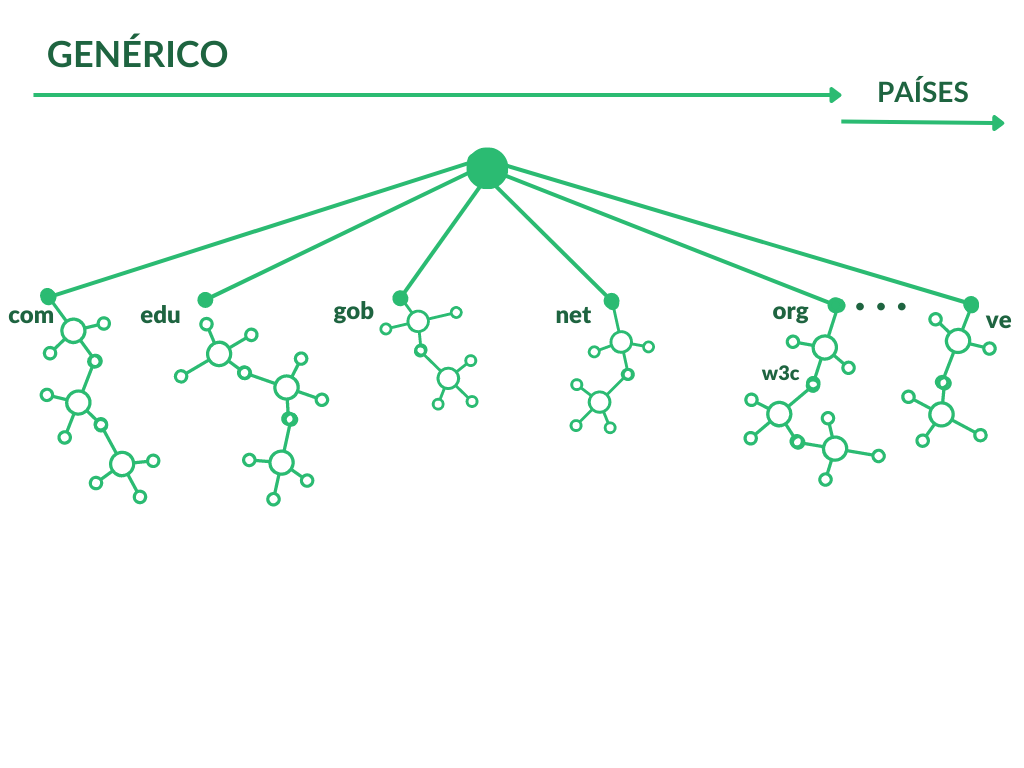
\includegraphics[width=0.8\linewidth]{1/DNS.png}
				\caption{Ejemplo de la divisi\'on del espacio de nombres del DNS original a zonas. Tomado de \cite{Steen2017}}
				\label{fig:DNSorg}
						\end{center}
			\end{figure}			
 			
		\end{itemize}
		
		\item[{Heterogeneidad}.] \index{heterogéneos} 
		Los sistemas distribuidos son heterogéneos, ya que se pueden construirse a partir de una variedad de redes, sistemas operativos, hardware informático y lenguajes de programación. Contemplar, por ejemplo, \gls{codigo movil} o \gls{maquina virtual}. El \gls{middleware} se usa para ocultar estar diferencias y permitir la comunicación y administración de datos entre aplicaciones distribuidas.
			
		%%%%%%%%%%%%%%%%%%%%%%%%%%%%%%%%%%
		
		\item[{Seguridad.}] \index{rendimiento} 
		\index{seguridad} \index{confiabilidad} 
		No es suficiente proporcionar acceso a servicios distribuidos. También es importante proporcionar garantías con respecto a cualidades asociadas con dicho acceso al servicio.  Ejemplos de estas caraterísticas incluyen parámetros relacionados con el rendimiento, seguridad y confiabilidad:  En un sistema distribuido, el cliente envia solicitudes de acceso a través de la red a un conjunto de servidores, o almacena sus datos en servicios en la nube. Ambos ejemplos requiere que se construyan aplicaciones seguras donde se protega la información que se envia por la red o la que se almacena en la nube. Este ultimo requerimiento es estudiado por la  criptografía de datos en  bases de datos en la nube.\index{ criptografía de datos}
		
	\end{description}

%%%%%%%%%%%%%%%%%%%%%%%
\section{Teorema CAP.}	\index{teorema CAP} El \gls{Teorema CAP}, inicialmente llamado como la conjetura CAP, recibi\'o el estatus de teorema cuando se proporcion\'o una prueba matem\'atica del concepto, ver \cite{Brewer2000}. 
 CAP establece que en un sistema distribuido, se puede cumplir como m\'aximo con dos de estas propiedades: \gls{consistencia}, \gls{disponibilidad} y \gls{tolerancia de particion}. 

\index{consistencia} En cuanto al concepto de \gls{consistencia}  en aplicaciones distribuidas, por ejemplo, si una empresa usa un servidor de base de datos de respaldo, cuando un usuario actualiza la cuenta de un cliente, esos mismos cambios se realizar\'ian en el servidor de respaldo.

\begin{figure} %
			\begin{center}
	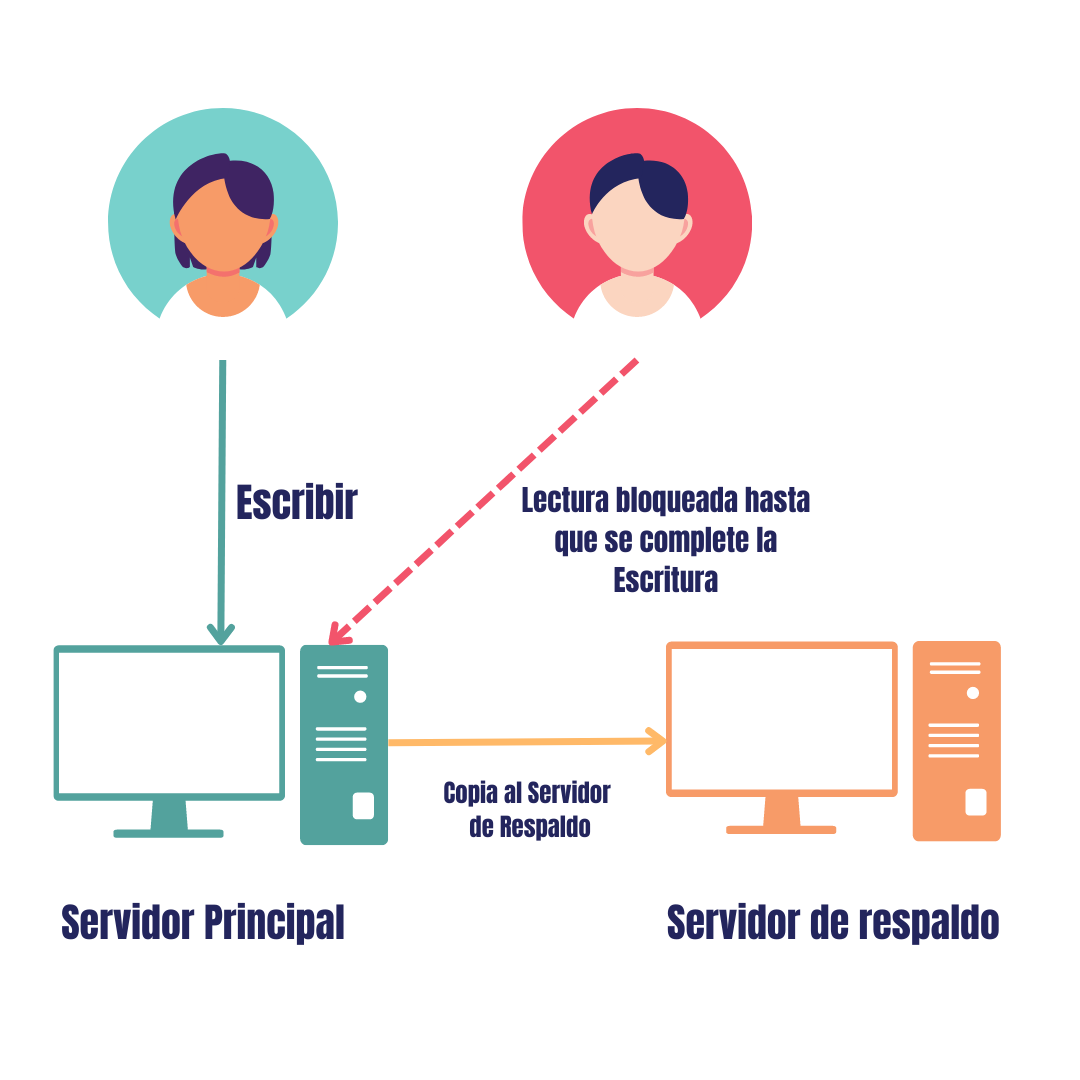
\includegraphics[width=0.8\linewidth]{1/Consistencia.png}
	\caption{Consistencia. Adaptado  de \cite{Sullivan2015} }
	\label{fig:marginCP}
			\end{center}
\end{figure}




Esto requeriría que la base de datos escribiera los datos dos veces: una vez en el disco usado por el servidor primario y luego una vez más en el disco usado por el servidor de respaldo en una operación conocida como confirmación de dos fases, ver Figura \ref{fig:marginCP}. 
Mientras se ejecuta la confirmación de dos fases, se bloquean otras consultas a los datos. Los datos actualizados no estarán disponibles hasta que finalice la confirmación de dos fases. Esto favorece la coherencia sobre la disponibilidad de los datos.


\index{disponibilidad} 
La \gls{disponibilidad} de datos se ilustra en el ejemplo del carrito de compras de comercio electr\'onico \cite{Sullivan2015}, 
donde es posible tener una copia de seguridad de los datos del carrito que no est\'e sincronizada con la copia principal. Los datos seguir\'ian estando disponibles si el servidor primario falla, pero los datos del servidor de respaldo ser\'ian inconsistentes con los datos del servidor primario si el servidor primario falla antes de actualizar el servidor de respaldo.  Ver la Figura \ref{fig:marginAP}.


\begin{figure}%
			\begin{center}
	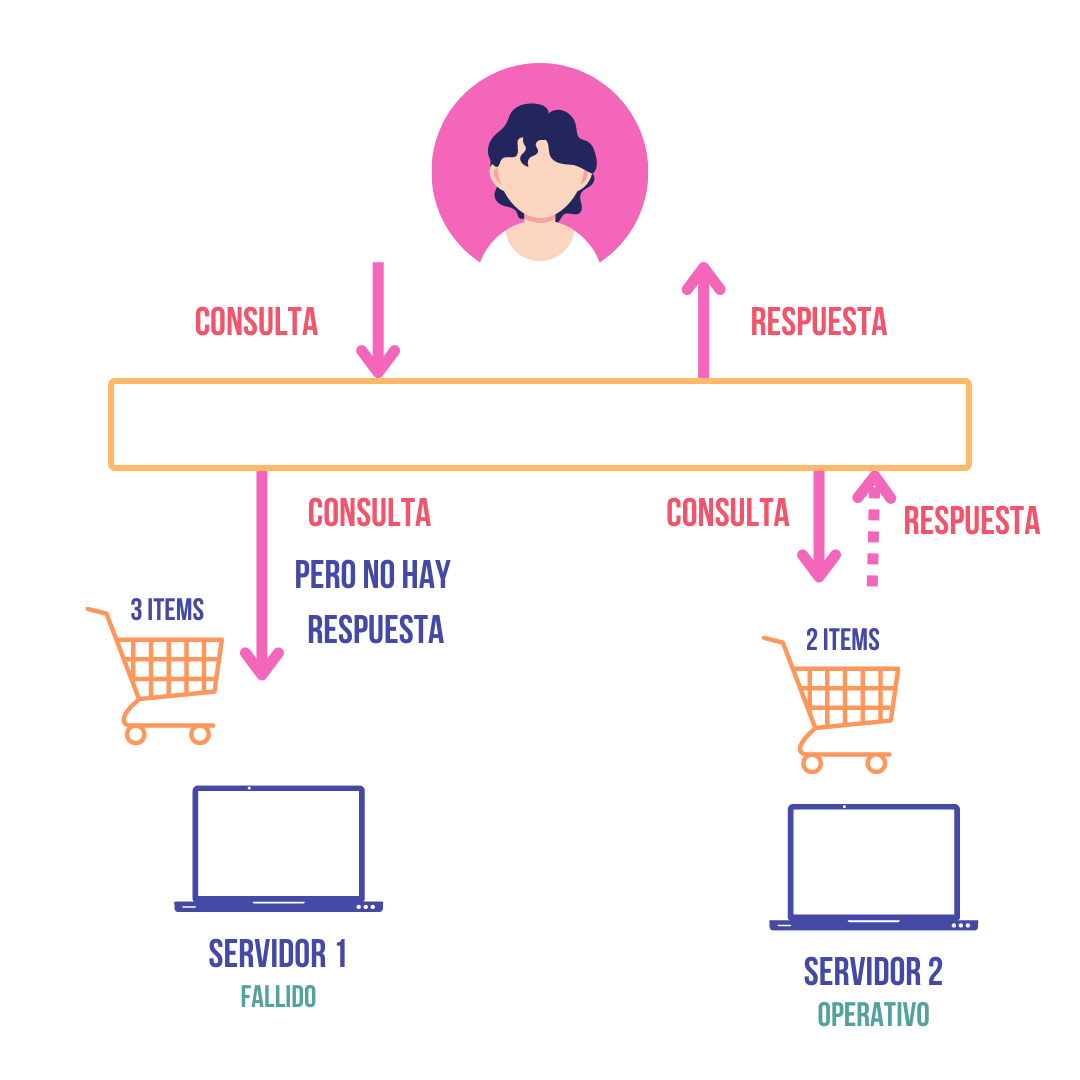
\includegraphics[width=0.8\linewidth]{1/Disponibilidad.png}
	\caption{Disponiblidad. Tomado de \cite{Sullivan2015} }
	\label{fig:marginAP}
			\end{center}
\end{figure}

El ejemplo m\'as simple de \gls{tolerancia de particion} es cuando el sistema continúa funcionando incluso si las máquinas involucradas en la prestación del servicio pierden la capacidad de comunicarse entre sí debido a que un enlace de red se cae (ver  Figura \ref{fig:marginToleranciaParticion}).

\begin{figure}[H]%
			\begin{center}
	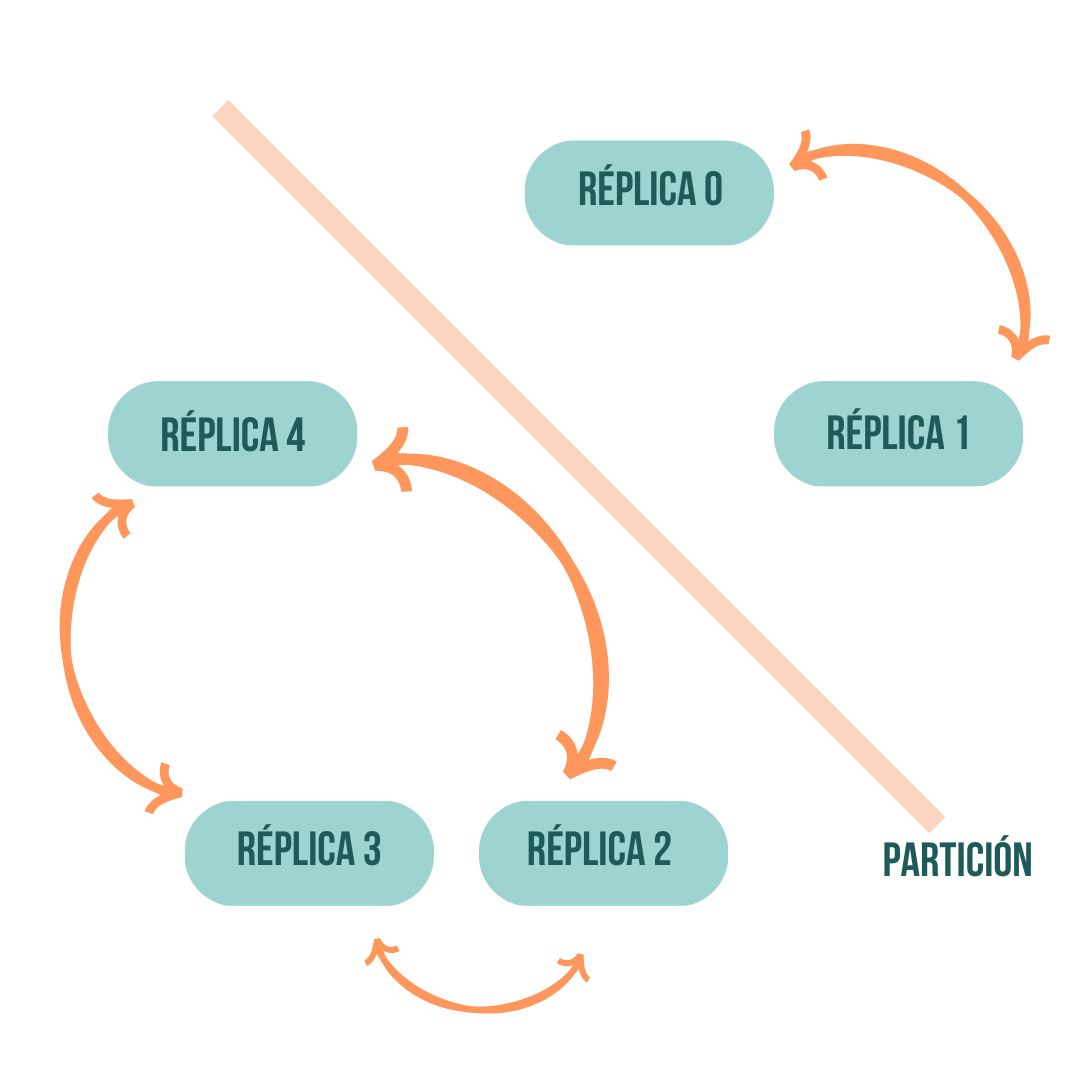
\includegraphics[width=0.8\linewidth]{1/ToleranciaParticion.png}
	\caption{Tolerancia a la Partici\'on. Adaptado de \cite{Limoncelli2014} }
	\label{fig:marginToleranciaParticion}
		\end{center}
\end{figure}
 
La Figura \ref{fig:marginTeoremaCAP} esquematiza estos conceptos y la relaci\'on entre ellos. Alli se resalta los puntos de intersecci\'on entre las propiedades definidas en el teorema, por ejemplo, \texttt{CA} es la intersecci\'on para los sistemas que cumplan la propiedad de consistencia y disponibilidad, \texttt{CP} son los sistemas con las propiedades de consistencia y toleracia a la partici\'on, y \texttt{AP} para las propiedades de disponibilidad y toleracia a la partici\'on.

Noten que la intersecci\'on entre los tres conceptos  no est\'a definida en la Figura \ref{fig:marginTeoremaCAP}. El principio \texttt{CAP} establece que no es posible construir un sistema distribuido que garantice los tres conceptos: consistencia, disponibilidad y tolerancia a la partici\'on. Se pueden lograr uno o dos de ellos, pero no los tres simultáneamente. Al utilizar un sistema distribuidos se debe tener en cuenta qu\'e principios puede garantizar, de acuerdo a su dise\~no. 

\begin{figure}%
			\begin{center}
	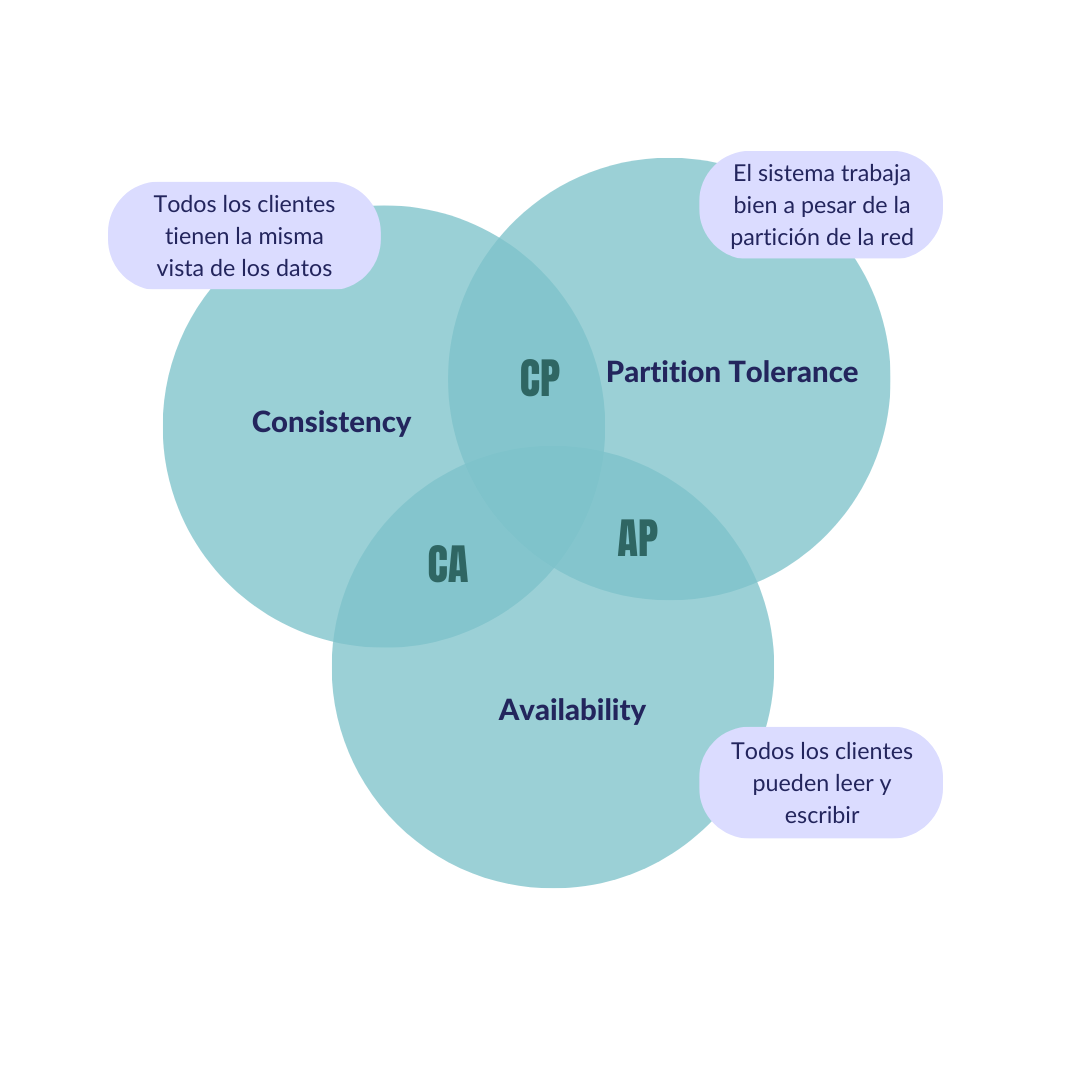
\includegraphics[width=0.8\linewidth]{1/TeoremaCAP1.png}
	\caption{ Relaci\'on entre conceptos del Teorema CAP. Adaptado  de \cite{Deka2017}}
	\label{fig:marginTeoremaCAP}
			\end{center}
\end{figure}


En el contexto de una aplicaci\'on de red social global, o un sistema de comercio electr\'onico mundial, la solución deseada es mantener la disponibilidad incluso si se sacrifica cierta consistencia entre los usuarios. Por otra parte, en el sistema financiero mundial, requiere  mantener la consistencia de los datos sobre la disponibilidad de los mismos, por tanto las actualizaciones podr\'ian requerir m\'as tiempo para su ejecuci\'on. 
%%
\begin{figure}
			\begin{center}
	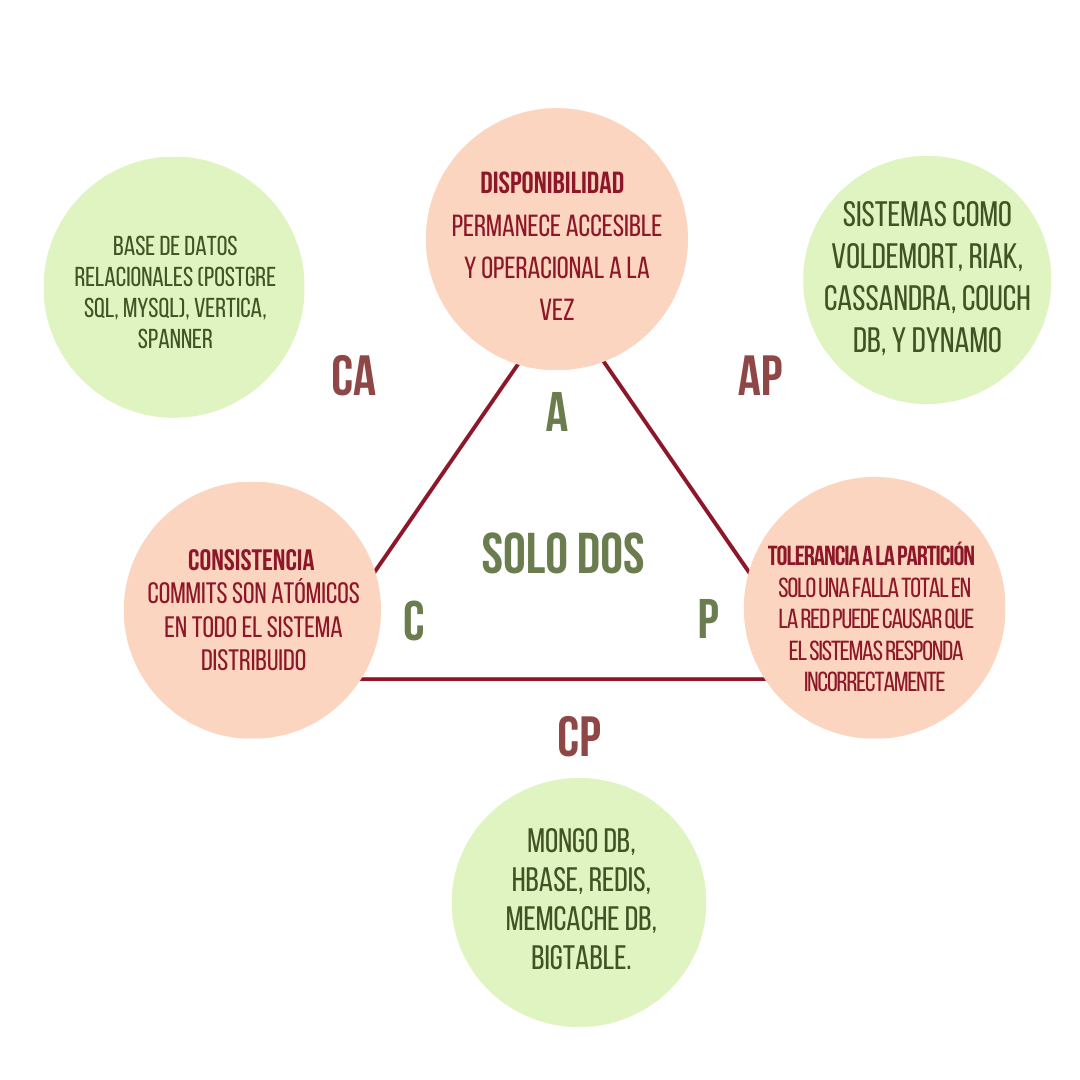
\includegraphics[width=0.8\linewidth]{1/TeoremaCAP.png}
	\caption {Significado del Teorema CAP.}
	\label{fig:TeoremaCAP}
			\end{center}
\end{figure}

En la Figura,  \ref{fig:TeoremaCAP} se muestra las propiedades del Teorema CAP y los tipos de aplicaciones que cumplen con estas propiedades.

%%%%%
	\section{Manejo de Fallas} \index{fallas} 
Los sistemas informáticos a veces fallan. Cuando estas ocurren, ya sea en  hardware o software, los programas pueden producir resultados incorrectos o  detenerse antes de que hayan completado el cálculo.  Las fallas en un sistema distribuido son parciales, es decir, algunos componentes fallan mientras otros continúan funcionando. Por lo tanto, el manejo de fallas es particularmente díficil. 

\index{técnicas contra fallas} Existen técnicas  para lidiar con fallas: detección de la ocurrencia de fallas, enmascaramiento de las fallas, tolerancia a las  fallas, recuperación luego de la ocurrencia de fallas y la redundancia de rutas, caminos o servidores para garantizar funcionamiento de las aplicaciones, a pesar de la fallas. 

En \cite{Gabrielson2019}  
destacan que las fallas en los sistemas distribuidos puede atribuirse a  la complejidad de la ingeniería de los mismos   y se deben a los siguientes motivos: 
	
\begin{tcolorbox}
	[colback=red!5!white,colframe=red!75!black,fonttitle=\bfseries,title=Retos en Sistemas Distribuidos ]
	Puede consultar este documento en \href{https://aws.amazon.com/es/builders-library/
		challenges-with-distributed-systems/} {Retos en SD}
\end{tcolorbox}

\begin{itemize}
	\item { Los ingenieros no pueden combinar las condiciones de error}. En su lugar, deben considerar muchas combinaciones de fallas. La mayoría de los errores pueden ocurrir en cualquier momento, independientemente de cualquiera otra condición de error, por lo que podrían combinarse entre ellos.
	
	\item {El resultado de cualquier operación de red puede ser DESCONOCIDO}. En cuyo caso es posible que la solicitud haya fallado, se haya procesado correctamente o se haya recibido pero no procesado.
	
	\item  {Los problemas distribuidos se producen en todos los niveles}. No solo en los equipos físicos de nivel bajo, sin tembi\'en, en los niveles lógicos del sistema distribuido.
	
	\item {Recursividad}.  Los problemas distribuidos empeoran en los niveles superiores del sistema, debido a la recursividad. 
	
	\item {Aparición del error}. Los errores distribuidos suelen aparecer mucho después de su implementación en un sistema.
	
	\item {Propagación del error}. Los errores distribuidos se pueden propagar en todo el sistema. 
	
	\item  {Origen de la falla}. Muchos de estos problemas provienen de las leyes físicas de las redes, que no se pueden cambiar.
\end{itemize}
%%%%%
Las fallas se caracaterizan como \cite{Coulouris2011}:
	
\begin{description}
	\item[Fallos por omisión] Los fallos clasificados como fallos por omisión se refieren a casos en los que un  proceso o el canal de comunicación no realiza las acciones que se supone que debe realizar
	
	\item [Fallos por omisión del proceso] El principal fallo por omisión de un proceso es que este se bloquee. Un proceso se ha bloqueado cuando se ha detenido y no  ejecutará ning\'un paso de su programa. En los sistemas s\'incronos  el  método de detección de estas fallas se basa en el uso de
	tiempos de espera - es decir, un método en el que un proceso permite un período de tiempo fijo para que  ocurra algo. 
	
	 
	\begin{tcolorbox}
		[colback=red!5!white,colframe=red!75!black,fonttitle=\bfseries,title=Fallas de omisión en sistemas síncronos]
		Por ejemplo, si los procesos $p$ y $q$ están programados para que $q$ pueda responder a un mensaje de $p$, y si el proceso $p$ no ha recibido respuesta del proceso $q$ en un tiempo máximo medido en el reloj local de $p$, entonces el proceso $p$ puede concluir que el proceso $q$ ha fallado.
	\end{tcolorbox}
	
	En un sistema asincrónico, un tiempo de espera puede indicar solo que un proceso no responde: puede que se haya bloqueado o sea lento, o los mensajes pueden que no han llegado.
	
	\item 	[Fallos de omisión de comunicación] Considere las primitivas de comunicación que envían y reciben mensajes. Un proceso $p$ realiza un envío insertando el mensaje $m$ en su buffer de mensaje saliente. El canal de comunicación transporta $m$ al búfer de mensajes entrantes de $q$. El proceso $q$ realiza una recepción tomando $m$ de su búfer de mensajes entrantes y lo entrega (ver Figura \ref{fig:proc-canal} ). Los búferes de mensajes entrantes y salientes son  proporcionado por el sistema operativo.
	
	\begin{figure}%
				\begin{center}
		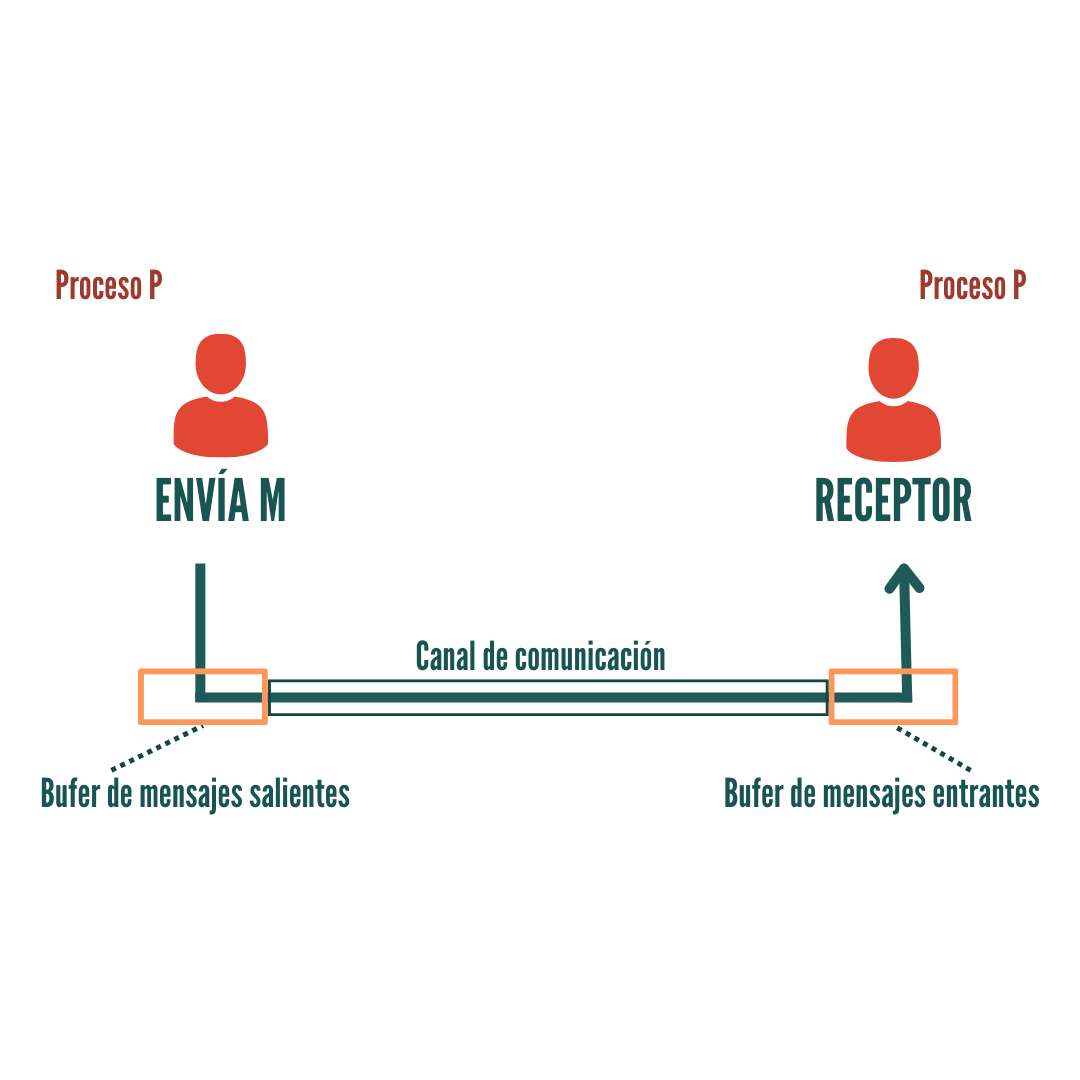
\includegraphics[width=0.8\linewidth]{1/procesos-canales.png}
		\caption{Procesos y canales.}
		\label{fig:proc-canal}
				\end{center}
	\end{figure}
%\end{description}

	El canal de comunicación produce una falla por omisión si no transporta	un mensaje del búfer de mensajes salientes de $p$ al búfer de mensajes entrantes de $q$. Esto  se debe a la falta de espacio en el búfer en el receptor o en una puerta de enlace intermedia, o por un error de transmisión de red, detectado por un  control de suma (\textit{check sum}) llevada con los datos del mensaje. 


	\item [Fallos arbitrarios]  El término fallo arbitrario o bizantino se utiliza para describir lo peor  falla de  semántica posible , en la que puede ocurrir cualquier tipo de error. Por ejemplo, un proceso puede establecer valores incorrectos en sus elementos de datos, o puede devolver un valor incorrecto en respuesta a un 	invocación.
	Un fallo arbitrario de un proceso es aquel en el que omite arbitrariamente el 	pasos de procesamiento o toma pasos de procesamiento no deseados.  
\end{description}
%%%%%%%%%%%%%%%%%%%%%%%%%%%%%%%%%%%%%%%

\begin{table}[h]\index{middleware}
	\footnotesize%
	\begin{center}
		\footnotesize
		 \begin{tabular}{p{0.18\textwidth}p{0.1\textwidth}p{0.6\textwidth}}
	%	\begin{tabular}{lll}
			\toprule
			Clase de Falla    &  Afecta   & Descripción  \\
			\midrule
			\quad Parada & Proceso & Proceso se detiene y permanece detenido.  Otros procesos pueden detectar este estado. \\
			
			\addlinespace
			\quad 	Bloqueo & Proceso & Proceso se detiene y permanece detenido.  Otros procesos no pueden  detectar este   estado.\\			\addlinespace
			
			\quad Omisión & Canal & Mensaje insertado en un búfer de mensajes  salientes no llega al  b\'ufer de mensajes   entrante del otro extremo  \\
			
			\addlinespace			
			\quad Omisión  Env\'io   & 	Proceso   & Proceso completa una operación de  envío pero el mensaje no se coloca     en su búfer de mensajes salientes.  \\
			
			\addlinespace		
			\quad Omisión  Recepci\'on & Proceso &  Mensaje se coloca en búfer  de mensajes   entrantes de un proceso, pero ese   proceso no lo recibe.  \\
			
			\addlinespace		
			\quad Arbitrario   (Bizantino) &  Proceso   & Proceso/canal muestra un comportamiento  arbitrario:  puede enviar/transmitir  mensajes arbitrarios en momentos arbitrarios o hacer omisiones; puede   detenerse  o tomar un  paso incorrecto. \\
			
			\addlinespace 
			\bottomrule
		\end{tabular}
	\end{center}
	\caption{Tipos de Errores. \\ Adaptado de \cite{Coulouris2011} }
	\label{tab:cat-middle}
\end{table}

\section{Falacias de los sistemas distribuidos}

Las falacias, también nombrado como trampas, son un conjunto de errores o falsas creencias que se cometen al diseñar y desarrollar un  sistemas distribuidos. 


\begin{tcolorbox}
	[colback=red!5!white,colframe=red!75!black,fonttitle=\bfseries,title=Historia de las falacias]
		Peter Deutsch, mientras trabajaba en la empresa Sun Microsystem, en la decada de los 90 propuso la lista de 7 falacias de la computación distribuida; posteriormente, en 1.994, James Gosling, fundador de Java,  añadió una más para finalmente ser conocida como las ocho falacias de los sistemas distribuidos.
\end{tcolorbox}


Las falacias son  \cite{Hoogen2004, Xu2022}:
\begin{description}
	\item \textbf{La red es fiable}.
	 Los sistemas no son inmunes a fallas: los servidores pueden estar fuera de servicio, la energia eléctrica puede fallar. Las aplicaciones deben estar construidas para sortear estas fallas.
	\item \textbf{La latencia es cero}. 
	La \gls{latencia} en redes pequeñas pueden considerarse casi cero; pero en las redes Wan, con servidores remotos, y usuarios alrededor del mundo, la latencia puede ser significativa.
	En estos casos, las aplicaciones deben tener cuidado con las respuestas tardías. Contemplar mecanismos para desechar las solicitudes, hacer reintentos de \gls{peticiones idempotentes}, como mecanismo de prevención de fallas.
	\item \textbf{El ancho de banda es infinito}.
	Así como el ancho de banda aumenta debido a las mejoras de la tecnología, el volúmen de datos se incrementa. Por ello,  podemos  tener problemas con el ancho de banda lo cual influiría en la degradación del rendimiento de la aplicación.
	\item \textbf{La red es segura}.
	Es un error no prestar atención a la seguridad de la aplicación. Las aplicaciones están expuestas a software maliciosos que pueden alterar las funcionalidades del software.
	\item \textbf{La topología no cambia}.
	La red está en cambio constante: nuevas direcciones ip, servidores, dispositivos, servicios, clientes,  entre otros. Los cambios en la topología influye sobre el ancho de banda y el rendimiento de las aplicaciones.	
	\item \textbf{Hay un solo administrador}.
	Un solo administrador es posible en redes pequeñas, pero para  grandes redes, distribuidas geograficamente y con distintos propietarios, esto no se cumple. 
	\item \textbf{El costo de transporte es cero}.
 	En la comunicación entre procesos distribuidos intervienen equipos, sistemas de balance de carga y ancho de banda; en cuanto a la comunicación entre las aplicaciones están involucrado el protocolo que se usa y como se serializa y deserializa.
	\item \textbf{La red es homogénea}.
	Una red homogénea es  pequeña con equipos bajo la misma tecnología, configuración y características. Pero en grandes redes esto no es así: allí se soportan una gran variedad de protocolos y dispositivos, aplicaciones con distintas necesidades y sistemas heterogéneos.
	
	
\end{description}


En la Figura \ref{fig:pitfall} se muestra un esquema con la síntesis de las ocho falacias de los sistemas distribuidos ya referidas.

\begin{figure}%
			\begin{center}
	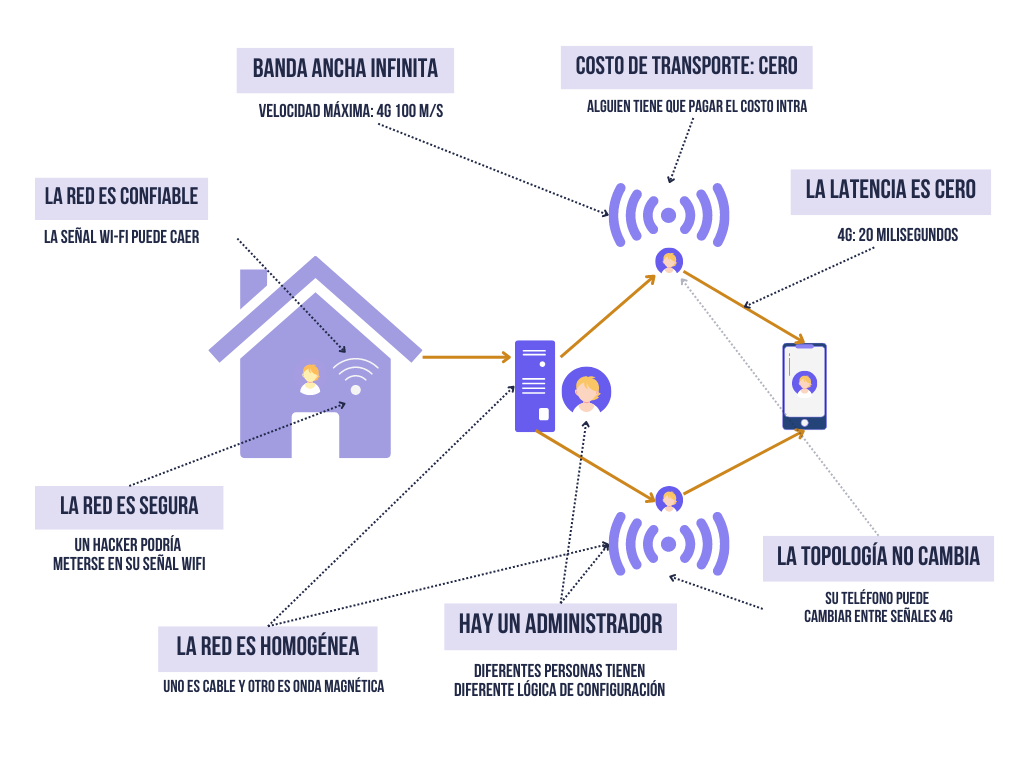
\includegraphics[width=0.8\linewidth]{1/pitfall.png}
	\caption{Fallas de los Sistemas Distribuidos. Adaptado de \cite{Xu2022} }
	\label{fig:pitfall}
			\end{center}
\end{figure}
%%%%
En resumen, diseñar una aplicación es una tarea que requiere considerar aspectos que están fuera del alcance del diseñador de la aplicación; por ello el proceso de diseño requiere que se haga un ejercicio de escenarios probables de funcionamiento para determinar si la aplicación puede seguir operando a pesar de las posibles escollos que encuentre.
%%%%%
%%\section{Ejercicios}
%\label{sec:ejercicios}

%%\begin{kaobox}[frametitle=Ejercicios ]
%%	\begin{enumerate}

%%\item  Proporcione cinco tipos de recursos de hardware y cinco tipos de datos o recursos de software que puedan ser compartido de manera útil. Dé ejemplos de cómo se comparten  en sistemas distribuciones en la practica.

%%\item Enumere los tres componentes principales de software que pueden fallar cuando un proceso cliente invoca un objeto en el  servidor, dando un ejemplo de falla en cada caso. Sugiera cómo los componentes se pueden fabricar para tolerar las fallas de los demás componentes.

%%\item Los recursos en la World Wide Web y otros servicios se nombran por URL. ?` Qué denotan las iniciales URL ? Dé ejemplos de tres tipos diferentes de recursos web que pueden nombrados por URL.

%%\item  Dé un ejemplo de una URL HTTP. Enumere los componentes principales de una URL HTTP, indicando  sus límites e ilustrando cada uno de ellos a partir de su ejemplo.  
%%\end{enumerate}

%%\end{kaobox}

%%%%%%%%%%%%%%%%%%%%%%%%%%%%%%%%%%%%%%%%%%%%%
\section{Caso de Estudio: Tecnología Web}
\index{caso de estudio!tecnología web}
\label{sec:caso-estudio:web}

La Web es un sistema abierto que se  caracteriza por \cite{Coulouris2011}: a) Su funcionamiento está basado en estándares de comunicación y contenido o en documentos que se publican e implementan libremente. Ejemplo, hay varios tipos de navegador,  implementado en distintas plataformas; así como  implementaciones de servidores web. b) La Web está abierta con respecto a los tipos de \gls{recursos} que se pueden publicar y compartir. Los navegadores están diseñados para adaptarse a nuevas funcionalidades de presentación de contenido en forma de aplicaciones auxiliares y complementos o \textit{plug-ins}.

La Web se basa en  componentes tecnológicos que son  estándares de la W3C, \cite{W3C2022} y que se describen en esta parte. Se presentan una introducción a las siguientes tecnolog\'ias que se usan  en la web: HTTP, HTML, CCS, JavaScript.

\subsection{HTTP}   \index{HTTP} 
HTTP (HyperText Transfer Protocol), \gls{HTTP} es el protocolo usado cuando se visita cualquier sitio web desde un navegador (\textit{browser}). Es un protocolo confiable que facilita la transferencia de información en la web. Esta característica de fiabilidad es  debido a que HTTP utiliza protocolos de transmisión de datos confiables, garantiza que sus datos no se dañarán ni se codificarán durante el tránsito, incluso cuando provengan del otro lado del mundo \cite{W3C2022}, \cite{Gourley2002},  \cite{Allen2017}.

 
\begin{tcolorbox}
	[colback=red!5!white,colframe=red!75!black,fonttitle=\bfseries,title=HTTP]
	Conozca m\'as de HTTP visitando este sitio  \href{https://www.w3.org/Protocols/}{HTTP}
\end{tcolorbox}

	\subsubsection{Clientes y Servidores Web}   \index{Hcliente}   \index{servidor web}
	El contenido de la  web está almacenado en un \gls{servidor web}. Los servidores web usan el protocolo HTTP, por lo que a menudo se les llama servidores HTTP. Estos servidores almacenan los datos de Internet y proporcionan los datos cuando los solicitan los clientes HTTP. Los clientes envían solicitudes HTTP a los servidores y los servidores devuelven los datos solicitados en respuestas HTTP, como se muestra en la Figura \ref{fig:CSweb}. 
	
	\begin{figure} %
				\begin{center}
		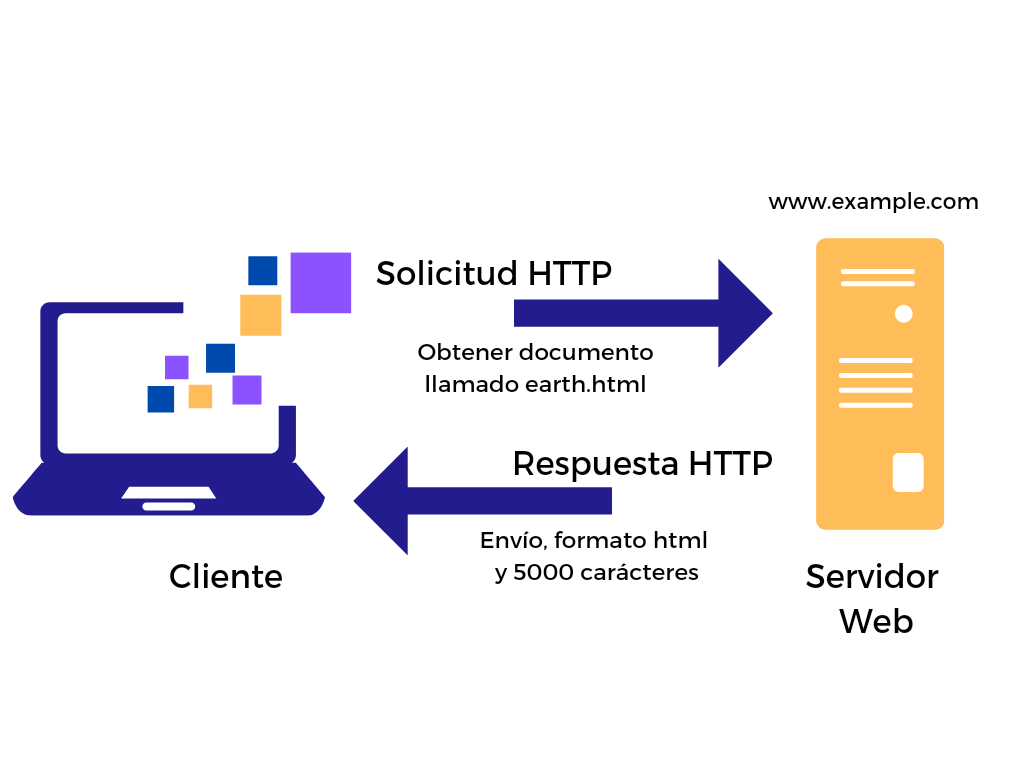
\includegraphics[width=0.8\linewidth]{1/Cliente-WebServer}
		\caption{Cliente y Servidor Web}
		\label{fig:CSweb}
				\end{center}
	\end{figure}
	
	
	\subsubsection{Recursos}   \index{recursos}
	Los servidores web alojan \gls{recursos}. Un recurso web es la fuente del contenido web. El tipo más simple de recurso web es un archivo estático en el sistema de archivos del servidor web: pueden ser archivos de texto, archivos HTML, archivos de Microsoft Word, archivos de Adobe Acrobat, archivos de imagen JPEG, archivos de película AVI o cualquier otro formato, ver Figura \ref{fig:CS-Recursos}.
	
		\begin{figure} [h] %
					\begin{center}
		\includegraphics[width=0.8\linewidth]{1/Recursos}
		\caption{Clientes, Servidor Web y Recursos }
		\label{fig:CS-Recursos}
				\end{center}
	\end{figure}

	Los recursos también pueden ser programas de software que generan contenido bajo demanda. Estos recursos de contenido dinámico pueden generar contenido en función de su identidad, de la información que haya solicitado o de la hora del día, por ejemplo videos, transacciones de comercio electrónico, transacciones bancarias, entre otros
	

	
	\subsubsection{MIME}  \index{MIME}
	Debido a que Internet alberga  miles de tipos de datos diferentes, HTTP etiqueta  cada objeto que se transporta a través de la Web con una etiqueta de formato de datos denominada tipo MIME. \gls{MIME} o \textit{Multipurpose Internet Mail Extensions}(en español, Extensiones de correo de Internet multipropósito) se diseñó originalmente para resolver los mensajes entre los sistemas de correo electrónico. HTTP lo adoptó para describir y etiquetar su propio contenido multimedia.
	
	Los servidores web adjuntan un tipo MIME a todos los datos de objetos HTTP. Cuando un navegador web recupera un objeto de un servidor, mira el tipo MIME asociado para ver si sabe cómo manejar el objeto. La mayoría de los navegadores pueden manejar cientos de tipos de objetos populares: mostrar archivos de imagen, analizar y formatear archivos HTML, reproducir archivos de audio a través de los parlantes de la computadora o iniciar software de complemento externo para manejar formatos especiales, entre otros
	
	\subsubsection{URL}
	 \index{URL} 
	 Los navegadores examinan las \gls{URL}	  para acceder a las correspondientes recursos. A veces, el usuario escribe una \textit{URL} en el navegador, o el  navegador busca la \textit{URL} correspondiente cuando el usuario hace clic en un enlace o selecciona uno de sus marcadores o \textit{bookmarks}.
	
 
	\begin{tcolorbox}
		[colback=red!5!white,colframe=red!75!black,fonttitle=\bfseries,title=URL]
			Conozca m\'as de URL visitando este sitio
		\href{https://www.w3.org/TR/url/}{URL}
	\end{tcolorbox}
	
	Ejemplo de las partes de un \textit{URL} se esquematiza en la Figura\ref{fig:URL-HowWork}: 
	
	\begin{figure} %
				\begin{center}
		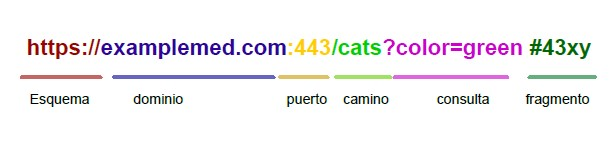
\includegraphics[width=0.8\linewidth]{1/URL.jpg}
		\caption{Partes de un URL }
		\label{fig:URL-HowWork}
				\end{center}
	\end{figure}

\begin{itemize}
	\item Esquema: es el protocolo usado para realizar la solicitud. Puede ser sin seguridad (http), encriptado (https) y para transferencia de archivos (ftp).
	\item Dominio: donde se envía la solicitud. En las solicitudes de tipo HTTP, el nombre del servidor de destino (host) se fija con este valor.
	\item Puerto: por defecto 80 para HTTP y 443 para HTTPS.
	\item Camino: es la dirección que se debe seguir en el servidor.
	\item Consulta: parámetros de consulta usados para especificar la página que se solicita.
	\item Fragmento: no es enviado en la solicitud al servidor. Se usa para buscar una etiqueta en el documento HTML o por un programa JavaScript en la página.
\end{itemize}
 

	\subsubsection{Transacciones HTTP} \index{transacción}
	Una transacción HTTP consta de un comando de solicitud (enviado del cliente al servidor) y un resultado de respuesta (enviado del servidor al cliente). Esta comunicación ocurre con bloques de datos formateados llamados mensajes HTTP, como se ilustra en la Figura \ref{fig:URL-tran}
	
	\begin{figure} %
				\begin{center}
		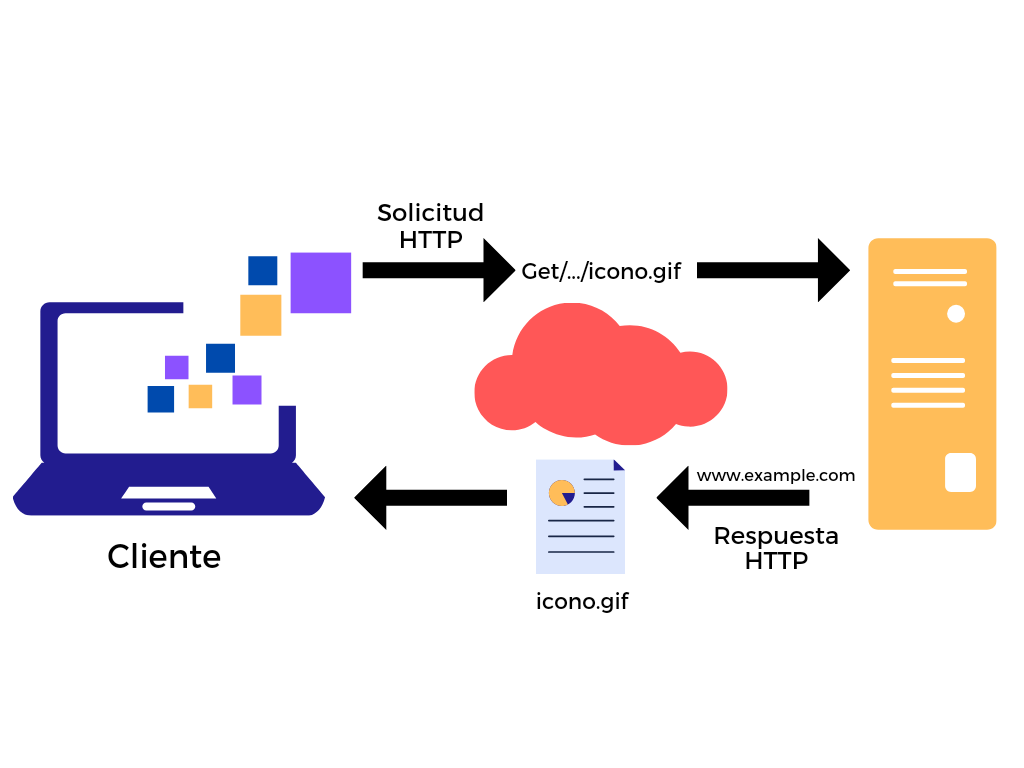
\includegraphics[width=0.8\linewidth]{1/URL-tran}
		\caption{Transacción HTTP }
		\label{fig:URL-tran}
				\end{center}
	\end{figure}
	
	\subsubsection{Métodos HTTP}  \index{métodos}
         HTTP proporciona  comandos de solicitud diferentes, llamados métodos HTTP. Cada mensaje de solicitud HTTP tiene un método. El método le dice al servidor qué acción realizar (obtener una página web, ejecutar un programa de puerta de enlace, eliminar un archivo, etc.). En la tabla \ref{tab:met-Http} hay una muestra de cuatro de ellos.

\begin{table}[H]
	\footnotesize%
	\begin{center}
		\footnotesize
		\begin{tabular}{ll}
			\toprule
			Método    &  Descripción    \\
			\midrule
			\quad GET  & Enviar nombre del recurso desde el servidor al cliente. \\  \\		\quad PUT  &  Almacenar datos del cliente en el recurso de destino. \\ \\	
			\quad DELETE & Borra  un recurso en específico. \\  \\	
			\quad POST & Envíar los datos del cliente a una aplicación en la \\ 
			\quad & puerta de enlace del servidor. \\				 
			\addlinespace 
			\bottomrule
		\end{tabular}
	\end{center}
	\caption{Métodos Http }
	\label{tab:met-Http}
\end{table}

\subsection{HTML}  
\index{HTML} 
El lenguaje de marcado de hipertexto, \gls{HTML} se utiliza para especificar el texto e imágenes que componen el contenido de una página web, y  cómo se colocan y formatean,  para su presentación al usuario. \textit{HTML} también se utiliza para especificar enlaces y  recursos que están asociados a ellos. \cite{W3C2022}

 
\begin{tcolorbox}
	[colback=red!5!white,colframe=red!75!black,fonttitle=\bfseries,title=HTML]
	Conozca m\'as de HTML visitando este sitio  \href{https://www.w3.org/html/}{HTML}
\end{tcolorbox}


A continuación, se muestra un fragmento  de texto \textit{HTML}, ver :

     \lstinputlisting[caption=Ejemplo programa en HTML]{C:/Users/virgi/OneDrive/Desktop/book/hello.html} \label{prog:HTML-1}


En el listado \ref{prog:HTML-1} del programa se puede distinguir las siguientes partes:
\begin{itemize}
	\item  La declaración <!DOCTYPE html> indica que este documento es un documento HTML5.
	\item El elemento <html> es el elemento raíz de una página HTML.
	\item El elemento <head> contiene metainformación sobre la página \textit{HTML}.
	\item El elemento <title> especifica un título para la página \textit{HTML} (que se muestra en la barra de título del navegador o en la pestaña de la página).
	\item El elemento <body> define el cuerpo del documento y es un contenedor de todos los contenidos visibles, como encabezados, párrafos, imágenes, hipervínculos, tablas, listas, etc.
	\item El elemento <h1> define un encabezado grande.
	\item El elemento <p> define un párrafo.
\end{itemize}

Un documento \textit{HTML} proporciona tres conceptos: etiqueta, atributo y valor.

\begin{itemize}
	\item Etiqueta: las etiquetas comparten el mismo formato: empiezan con el signo menor que "<" y terminan con el signo mayor que ">". 	Por ejemplo, el elemento html tiene dos etiquetas: etiqueta de inicio <html>   del documento \textit{HTML} y la etiqueta de cierre \textit{</html>} que indica el final del documento \textit{HTML}.
	
	\item Atributo: Son las propiedades que se le pueden asignar a los elementos. Su formato es  \textit{<elemento atributo='valor'> ... </elemento> }.
	\item Valor: es la cualidad asignada al atributo. Ejemplo:  \textit{<html lang='es'> ... </html>} indica el idioma en que está escrito el documento (lang) y el valor asignado es un código de idioma ("es" para el español).
\end{itemize}

Para ejecutar un documento HTML, solo abra el documento con el navegador de su preferencia;
obtendría la siguiente Figura \ref{fig:HTML-1}

	\begin{figure} %
				\begin{center}
	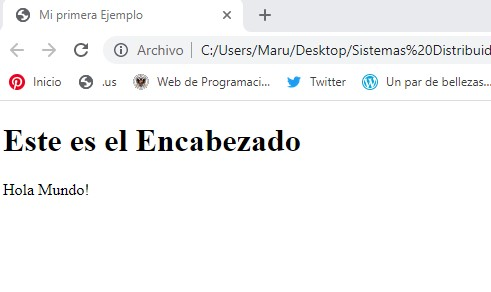
\includegraphics[width=0.8\linewidth]{1/HTML-1.jpg}
	\caption{Hola Mundo}
	\label{fig:HTML-1}
			\end{center}
\end{figure}

\subsubsection{CSS} 
\index{CSS}
\textit{CSS} es la abreviación para referirse a las hojas de estilo en cascada (Cascading Style Sheets), estas se utilizan  para dar formato a las páginas web. Por ejemplo, \gls{CSS}
se puede utilizar para definir el color, el ancho, la altura, los márgenes, la opacidad, el relleno, entre otros atributos. etc.
Usemos el programa \ref{prog:HTML-1} para mostrar como podemos incluir formato en la p\'agina Hola Mundo. 

 Escriba el programa \ref{prog:css-1} y guardelo como \textit{app.css} en una carpeta  llamada \textbf{css}. El programa tiene tres parte: la primera asigna color al fondo de la página, la segunda parte esta dedicada a colorear los elementos marcados con la etiqueta \textit{<h1>}, y en la tercera parte se le asigna color a los elementos contenidos en la etiqueta \textit{<p>}.
 
     \lstinputlisting[caption=Hoja de estilo app.css]{C:/Users/virgi/OneDrive/Desktop/book/html/css/app.css} \label{prog:css-1}
    
     Incluya en el programa Hola Mundo  la siguiente línea  \textit{<link rel="stylesheet" href="css/app.css">}, dabajo de la etiqueta \textit{title}
     
     El programa Hola Mundo modificado se muestra en \ref{prog:Hello2}. 
     
    \lstinputlisting[caption= Hola Mundo con llamada a css]{C:/Users/virgi/OneDrive/Desktop/book/html/hello.html} \label{prog:Hello2}
 
 El programa Hola Mundo tiene ahora la siguiente salida, como puede ver en la Figura \ref{fig:HTML-2}. 
 
 \begin{figure} %
 			\begin{center}
 	
\includegraphics[width=0.8\linewidth]{1/HTML-2.jpg}
 	\caption{Hola Mundo con hoja de estilo css}
 	\label{fig:HTML-2}
 			\end{center}
 \end{figure}


 Hay tres formas de implementar una hoja de estilo \textit{CSS} en un programa \textit{HTML}: interno, externo, y archivo en línea. 
\begin{itemize}
	\item Interno en una etiqueta: se añade una etiqueta \textit{<etiqueta style="">} en el programa \textit{HTML} con la definición del estilo. 
	\item Externo: En la sección \textit{<head>} de la página se puede incluir una etiqueta \textit{<style>} que integre todas las reglas de estilo de la página.
	\item Archivo: Mediante la etiqueta \textit{<link>} se puede incluir un fichero externo que incluya todas las reglas.
\end{itemize}
 
 
 En el primer caso sólo se deben especificar los estilos que se aplicarán al elemento en cuestión. Mientras que en los otros dos es necesario especificar, además, a qué elementos de la página se aplicarán los estilos. El último caso es el  mostrado en esta sección. 
 
  
 
 \begin{tcolorbox}
 	[colback=red!5!white,colframe=red!75!black,fonttitle=\bfseries,title=CSS]
 		Puede ampliar el tema de CSS y crear otros estilos revisando esta página  \href{https://www.w3.org/Style/CSS/}{CSS}
 \end{tcolorbox}
 
 Puede ampliar  este tópico y crear otros estilos revisando la siguiente bibliografía referida en la nota al margen del texto y en \cite{DuRocher2021,Shaw2017}.
 

 
\subsubsection{XHTML} 
\index{XHTML}

\textit{XHTML} significa lenguaje de marcado de hipertexto extensible (eXtensible HyperText Markup Language). Es una versión diferente de \textit{HTML}, basada en \textit{XML}. \textit{XHTML} se usa para hacer páginas web y tiene una forma muy específica de escribirse para que sea correcto y sin errores. \textit{XHTML} también distingue entre mayúsculas y minúsculas. Las etiquetas están escritas en minúsculas y deben cerrarse. El orden de las etiquetas también debe estar en el orden correcto para que la información salga correcta. Hay tres secciones principales de XHTML que consisten en una \textit{declaración de declaración}, una \textit{declaración principal} y un \textit{cuerpo}, \cite{Pfaffenberger2004,Musciano2002}.

Un documento \textit{XHTML} se compone de cuatro componentes:

\begin{itemize}
	\item Definición de tipo de documento (DTD): La DTD describe el idioma o la gramática en la que se ha codificado el texto. Es opcional en \textit{HTML}, pero en \textit{XHTML} es requerido.  Pueden ser de tipo \textit{Strict} (no soporta etiquetas antiguas y el código debe estar escrito correctamente), \textit{Transitional} (como XHTML Strict DTD, pero las etiquetas en desuso están permitidas) y \textit{Frameset}(la única DTD XHTML que soporta Frameset, que divide el espacio del documento) donde haya sido insertado, y permite la carga de otros documentos en cada espacio.
	\item Contenido de texto: los encabezados y párrafos que aparecen en la página.
	\item Referencias: contenido avanzado como enlaces e imágenes.
	\item Mark-Up: Instrucciones sobre cómo se debe mostrar el contenido.
\end{itemize}
Cada uno de estos componentes  puede guardarse en formato de texto y verse en cualquier navegador.  
Para adaptar un documento HTMl a XHTML solo debe agregar al inicio del programa el DTD, ver programa \ref{prog:XHTML}
 
     \lstinputlisting[caption=Hola Mundo con HTML y CSS]{C:/Users/virgi/OneDrive/Desktop/book/html/xhtml/hello.html} \label{prog:XHTML}
     
     La diferencia de \textit{XHTML} versus \textit{HTML} son las siguientes:
     
     \begin{itemize}
     	\item <!DOCTYPE> es obligatorio
     	\item El atributo xmlns en <html> es obligatorio
     	\item <html>, <head>, <title> y <body> son obligatorios
     	\item Los elementos siempre deben estar correctamente anidados
     	\item Los elementos siempre deben estar cerrados.
     	\item Los elementos siempre deben estar en minúsculas
     	\item Los nombres de los atributos siempre deben estar en minúsculas.
     	\item Los valores de los atributos siempre se deben citar.
     	\item La minimización de atributos está prohibida.
     \end{itemize}

 Est proporciona las siguientes ventajas en el uso de \textit{XHTML}: 1) Se pueden incorporar elementos de distintos espacios de nombres XML (como MathML y Scalable Vector Graphics). 2)  Un navegador no necesita implementar heurísticas para interpretar el texto por lo que el \textit{parser} puede ser mucho más sencillo. Y 3) Se pueden utilizar fácilmente herramientas creadas para procesamiento de documentos XML genéricos (editores, XSLT, entre otras).

\subsubsection{Páginas Dinámicas}  
\index{script} \index{página dinámica} \index{página estáticas} 

Las páginas dinámicas  \cite{Hoffer2016,Limoncelli2014} son páginas \textit{HTML} generadas a partir de lenguajes de programación \textit{(\gls{scripts})} que son ejecutados en el propio servidor web. A diferencia de otros scripts, como  \textit{JavaScript}, que se ejecutan en el propio navegador del usuario, los scripts en el lado del servidor (\textit{'Server Side' scripts})  generan un código \textit{HTML} desde el propio servidor web. 

Por su parte, las páginas estáticas no son  páginas sin movimientos, son páginas que permanece tal y como fue diseñada. Sin embargo, una página web estática también puede proporcionar una experiencia de usuario "en vivo", "dinámica" o "interactiva". El contenido (texto, imágenes, campos de formulario, etc.) en una página web puede cambiar, en respuesta a diferentes contextos o condiciones.

Estos comportamientos se explican de la siguiente manera:

\begin{itemize}
	\item \gls{pagina estatica}. Uso de secuencias de comandos del lado del cliente para cambiar los comportamientos de la interfaz dentro de una página web específica, en respuesta a las acciones del ratón o \textit{mouse}, o del teclado o en eventos de tiempo específicos. En este caso, el comportamiento dinámico ocurre dentro de la presentación. 
	\item \gls{pagina dinamica}. Uso de secuencias de comandos en el lado del servidor para cambiar la fuente de la página proporcionada entre páginas, ajustando la secuencia o recarga de las páginas web o el contenido web proporcionado al navegador. Las respuestas del servidor pueden estar determinadas por condiciones tales como datos en un formulario HTML publicado, parámetros en la URL, el tipo de navegador que se utiliza, el paso del tiempo o una base de datos o el estado del servidor.
\end{itemize}

Sin embargo, si un usuario  que envía una solicitud de página web no sabe si la solicitud que se envía se está devolviendo a una página web estática o una página web cuyo contenido es una mezcla de información estática y dinámica recuperada de una base de datos \cite{Hoffer2016}.
En la Figura \ref{fig:sol-pag-din} se ilustra cómo es el tratamiento de la información cuando se realiza un requerimiento al servidor.

 \begin{figure} %
 			\begin{center}
	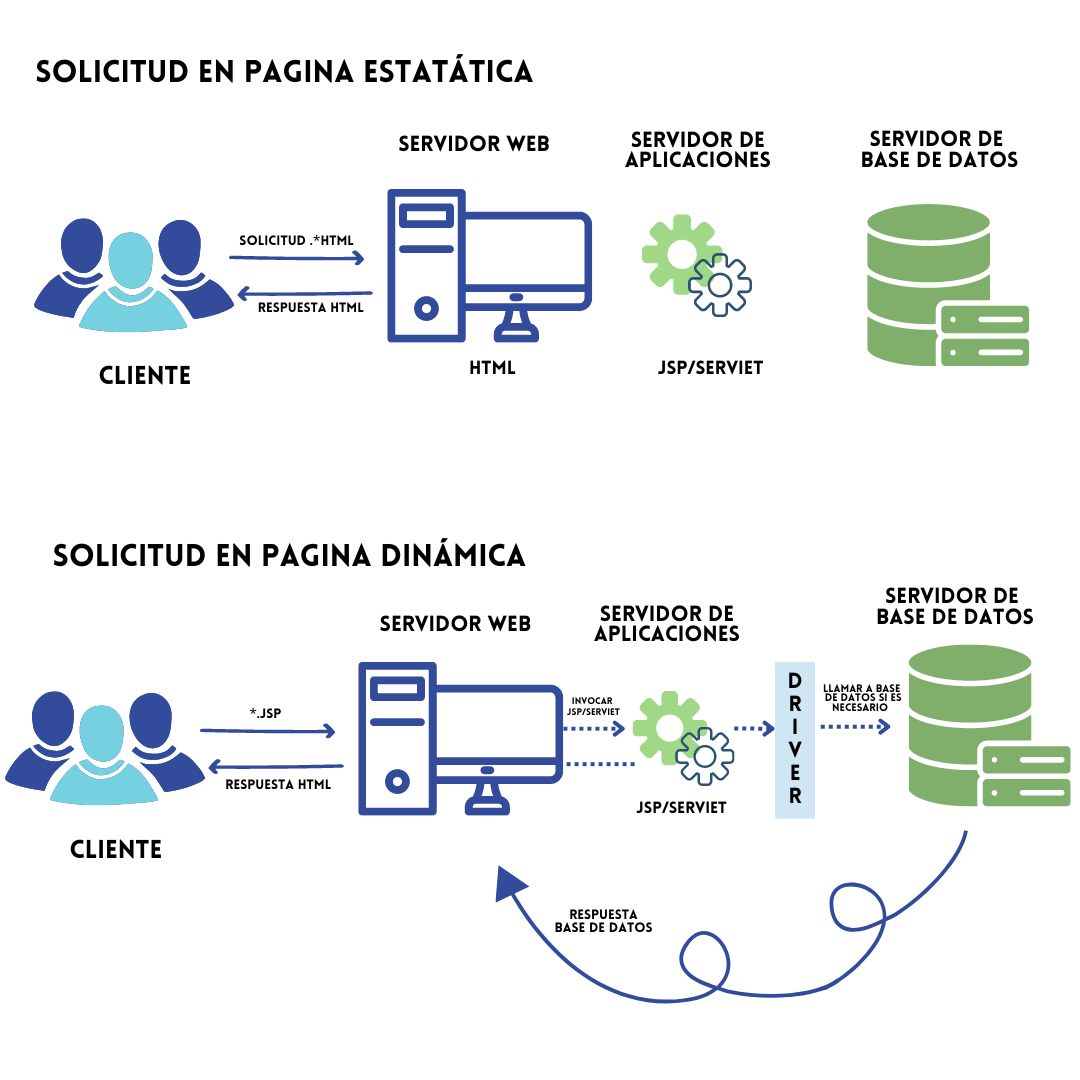
\includegraphics[width=0.8\linewidth]{1/sol-pag-dinamica}
	\caption{Solicitud página estática y página dinámica. Adaptado de \cite{Hoffer2016}}
	\label{fig:sol-pag-din}
			\end{center}
\end{figure}


%Este código HTML puede ser modificado -por ejemplo- en función de una petición realizada por el usuario en una Base de Datos. Dependiendo de los resultados de la consulta en la Base de Datos, se generará un código HTML u otro, mostrando diferentes contenidos.  \cite{Owen2022}.   Gran parte de la experiencia de los usuarios en la Web es el de interactuar con los servicios en lugar de recuperar datos. Por ejemplo, cuando se compra un artículo en una tienda en línea, el usuario  completa un \gls{formulario web} para proporcionar datos personales o para especificar  lo que se desea comprar.  Cuando el usuario envía el formulario, el navegador envía una solicitud \textit{HTTP} a un servidor web, que contiene los valores que el usuario ha ingresado. 

%Dado que el resultado de la solicitud depende de la entrada del usuario, el servidor debe procesar la entrada del usuario. Por lo tanto, la \textit{URL} o su componente inicial designa un 	programa en el servidor. 	Si la entrada del usuario es un conjunto  pequeño de 	parámetros,  se envía como el componente de consulta de la \textit{URL}, utilizando m\'etodo \textit{GET} o alternativamente, se envía como datos adicionales en la solicitud utilizando el m\'etodo \textit{POST}.
%%%%%
\paragraph{JavaScript} 
\index{JavaScript}

Javascript es el lenguaje de programación de la Web \cite{Flanagan2006}. \gls{JavaScript} es  un lenguaje interpretado que es ejecutado por el navegador que utilizamos para ver las páginas. Eso hace posible  desarrollar páginas dinámicas de muy diverso tipo, desde generadores de HTML, comprobadores de formularios, hasta programas que gestionen las capas de una página .  

También se puede usar para actualizar partes del contenido de una página web sin
obtener una versión completamente nueva de la página y volver a renderizarla. Estas actualizaciones dinámicas pueden ocurrir ya sea debido a una acción del usuario , o cuando
el navegador adquiere nuevos datos del servidor que suministró la página web. 
En este ultimo caso,  el momento de la llegada de los datos no está relacionado con ninguna acción del usuario en el propio navegador, por ello se denomina asíncrono. Una técnica conocida como \textit{AJAX}  se utiliza en tales casos.

 
\begin{tcolorbox}
	[colback=red!5!white,colframe=red!75!black,fonttitle=\bfseries,title=JavaScript]
	Una breve historia de JavaScript en este vídeo \href{https://www.youtube.com/watch?v=i18gWXhv5aA}{JavaScript}
\end{tcolorbox}


\paragraph{AJAX}
\index{AJAX}
 

\textit{Ajax} (Asynchronous JavaScript and XML) \cite{Asleson2005} se refiere a un grupo de tecnologías que se utilizan para desarrollar aplicaciones web. Al combinar estas tecnologías, las páginas web son más receptivas puesto que los paquetes  de datos que se intercambian con el servidor y las páginas web no se vuelven a cargar cada vez que un usuario realiza un cambio de entrada. 

El término \textit{Ajax}  proviene de la agrupación de las tecnologías que lo sustentan \cite{Gehtland2006}: 
\begin{enumerate}
	\item un canal de comunicación asíncrono entre el navegador y el servidor.
	\item JavaScript y XML.
\end{enumerate}

\textit{Ajax} se compone de las siguientes tecnologías:

\begin{itemize}
    \item Presentación basada en estándares usando XHTML y CSS.
    \item Visualización dinámica e interacción utilizando el \textbf{Modelo de Objetos del Documento} (\gls{DOM}, Document Object Model) del navegador. 
	\item  Intercambio y manipulación de datos mediante XML y XSLT.
	\item Recuperación asíncrona de datos usando el objeto \gls{XMLHttpRequest}.
	\item JavaScript que une todo.
\end{itemize}
%%%%
En la Figura \ref{fig:AJAX} se muestra como encajan estas tecnologías \cite{Crane2005}.  JavaScript  mantiene unida la aplicación, definiendo el flujo de trabajo del usuario y la lógica de negocio. La interfaz de usuario se manipula y actualiza
mediante el uso de JavaScript para gestionar el modelo de objetos de documento (DOM), redibujando y reorganizando continuamente los datos presentados a los usuarios y procesando sus interacciones basadas en el mouse y en el teclado. Las hojas de estilo en cascada (CSS) brindan una apariencia consistente a la aplicación  para la manipulación  del DOM. El objeto \textit{XMLHttpRequest}  se utiliza para hablar con el servidor de forma asincrónica, ejecutando las solicitudes de los usuarios y la obtención de datos actualizados mientras el usuario continúa operando. 

 \begin{figure} %
 			\begin{center}
	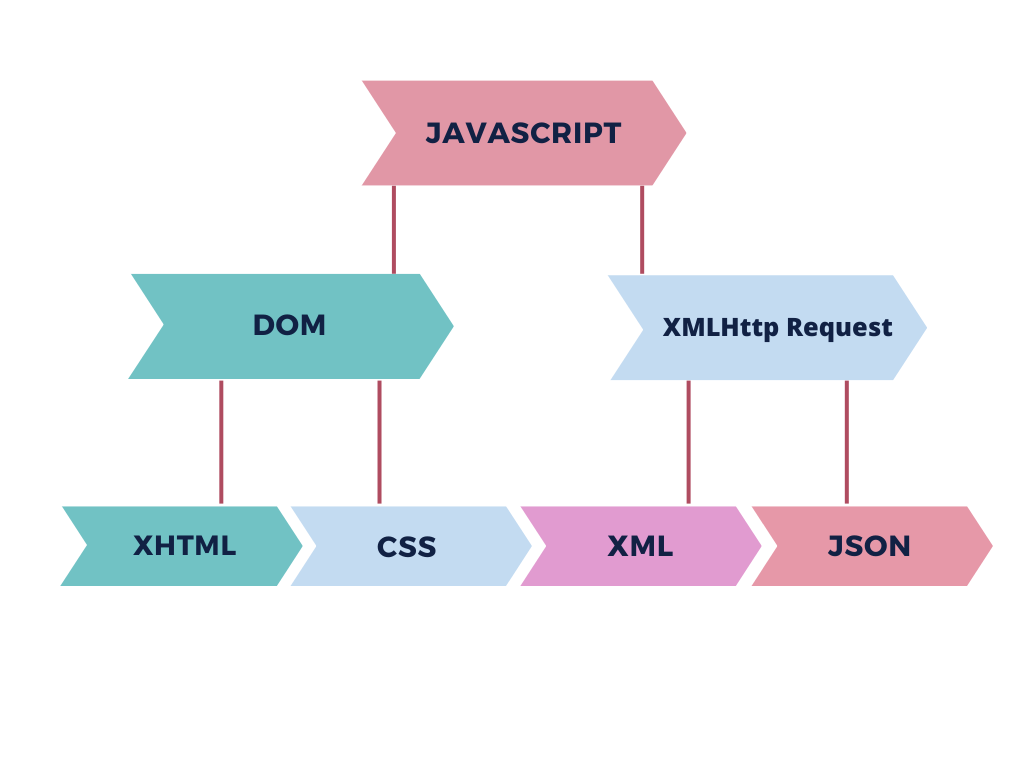
\includegraphics[width=0.8\linewidth]{1/AJAX}
	\caption{Componentes de AJAX. Adaptado de \cite{Crane2005}}
	\label{fig:AJAX}
		\end{center}
\end{figure}


En una aplicación web tradicional, las solicitudes HTTP que se inician mediante la interacción del usuario con la interfaz web, se envía a un servidor web. El servidor web procesa la solicitud y devuelve una página HTML al cliente. Durante el transporte HTTP, el usuario no puede interactuar con la aplicación web.
Esta técnica tradicional para crear aplicaciones web funciona correctamente, pero cuando se realizan peticiones continuas al servidor, el usuario debe esperar a que se recargue la página con los cambios solicitados.

Ajax define un método de iniciar un cliente con la comunicación del servidor sin recargas de páginas. Proporciona una forma de permitir actualizaciones de página parciales mediante la creación de un elemento intermedio entre el cliente y el servidor. En la Figura \ref{fig:AJAX-how} se visualiza un ejemplo de una interacción AJAX \cite{Asleson2005}. 
\begin{enumerate}
	\item  Un evento del lado del cliente desencadena un evento Ajax. Puede ser desde un simple evento onchange hasta alguna acción específica del usuario.
	
	\item Se crea una instancia del objeto XMLHttpRequest. Con el método open(), se configura la llamada: la URL  junto con el método HTTP deseado, generalmente GET o POST. La solicitud  se activa a través de una llamada al método send().
	
	\item Se realiza una solicitud al servidor. Esto podría ser una llamada a un servlet, un script CGI o cualquier 	técnica del lado del servidor.
	\item El servidor puede hacer cualquier cosa que se le ocurra, incluso acceder a una base de  de datos u	otro sistema
	\item La solicitud se devuelve al navegador. El tipo de contenido se establece en tipo texto/xml ( objeto XMLHttpRequest solo puede procesar resultados del tipo texto/html). La respuesta podría incluir ser más compleja e incluir JavaScript, manipulación DOM,
	u otras tecnologías relacionadas.
	\item En este ejemplo, el objeto XMLHttpRequest llama a la función callback() cuando regresa el procesamiento. Esta función verifica la propiedad readyState en el objeto XMLHttpRequest y luego mira el código de estado devuelto por el servidor. Si todo es como se esperaba, la función de devolución de llamada podría hacer algo en el  lado del cliente.
\end{enumerate}


\begin{figure} %
			\begin{center}
		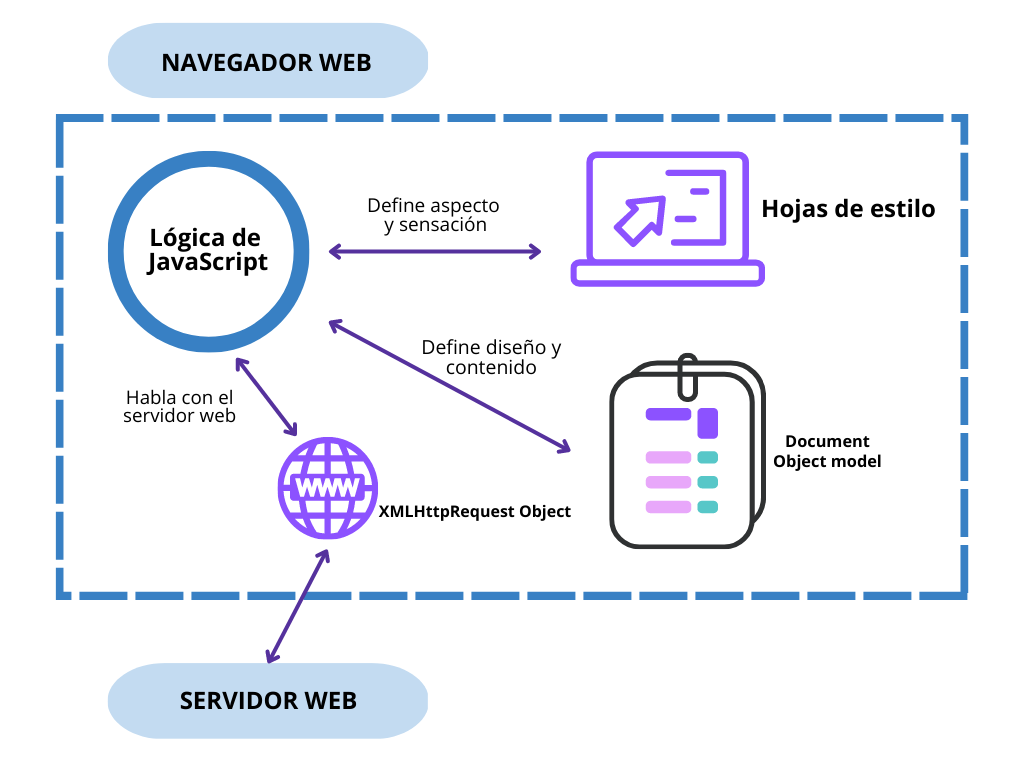
\includegraphics[width=0.8\linewidth]{1/AJAX-log}
	\caption{Una interacción AJAX. Adaptado de \cite{Asleson2005}  }
	\label{fig:AJAX-how}
			\end{center}
\end{figure}

Este comportamiento es distinto de una interacción solicitud-respuesta. Desde la perspectiva del usuario de página web, significa  una mejora de la interacción con una aplicación web, que proporciona al usuario más control de su entorno, y que es similar a la de una aplicación de escritorio.



%%%%%%%

%En resumen, \textit{HTML} es una herramienta para organizar, categorizar y estructurar contenido. \textit{CSS} brinda la capacidad de cambiar la apariencia y la forma de esa estructura para brindar una mejor experiencia visual; los estilos \textit{CSS} desarrollan el contenido y mejoran la experiencia del usuario. Por su parte,  \textit{HTML} crea la columna vertebral de la información en una página web.